\begin{titlepage}
\begin{center}

\includegraphics[scale=0.15]{Documents/niser.png}
\line(1,0){400}\\
[2mm]
\begin{large}
\textbf{\huge Integrator, Differentiator and Active Pass Filter}\\ 
\end{large}
\line(1,0){250}\\
[5cm]
\large MAITREY SHARMA\\
\small (1911093)\\
[4.5cm]
Second Year Integrated M.Sc.\\
\textbf{School of Physical Sciences}\\
\textbf{National Institute of Science Education and Research, Bhubaneshwar}\\
\small March 10, 2021
\end{center} 
\end{titlepage}
\newpage
\section{Aim}
\begin{itemize}
    \item To study Op-Amp as a differentiator.
    \item To study Op-Amp as an integrator.
\end{itemize}
\section{Apparatus}
\noindent Op-Amp IC741, resistors, oscilloscope, DC voltage source, function generator, digital storage oscilloscope, breadboard, multimeters and connecting wires.
\section{Theory}
\noindent So far the Op-Amps we have dealt with had a negative feedback, with only resistors being part of the loop. We can also construct RC circuits involving Op-Amps just like the RC-coupled transistor amplifiers.
\par
\begin{center}
    \textbf{\large Integrator Amplifier}
\end{center}
\noindent The \textbf{\emph{Integrator Amplifier}} is a configuration of an RC-coupled Op-Amp circuit which performs the mathematical operation of \emph{integration}, that is, we can cause the output to respond to changes in the input voltage over time and the integrator amplifier produces a voltage output which is proportional to that of its input voltage with respect to time. In other words, the magnitude of the output signal is determined by the length of time a voltage is present at its input as the current through the feedback loop charges or discharges the capacitor.
\begin{center}
    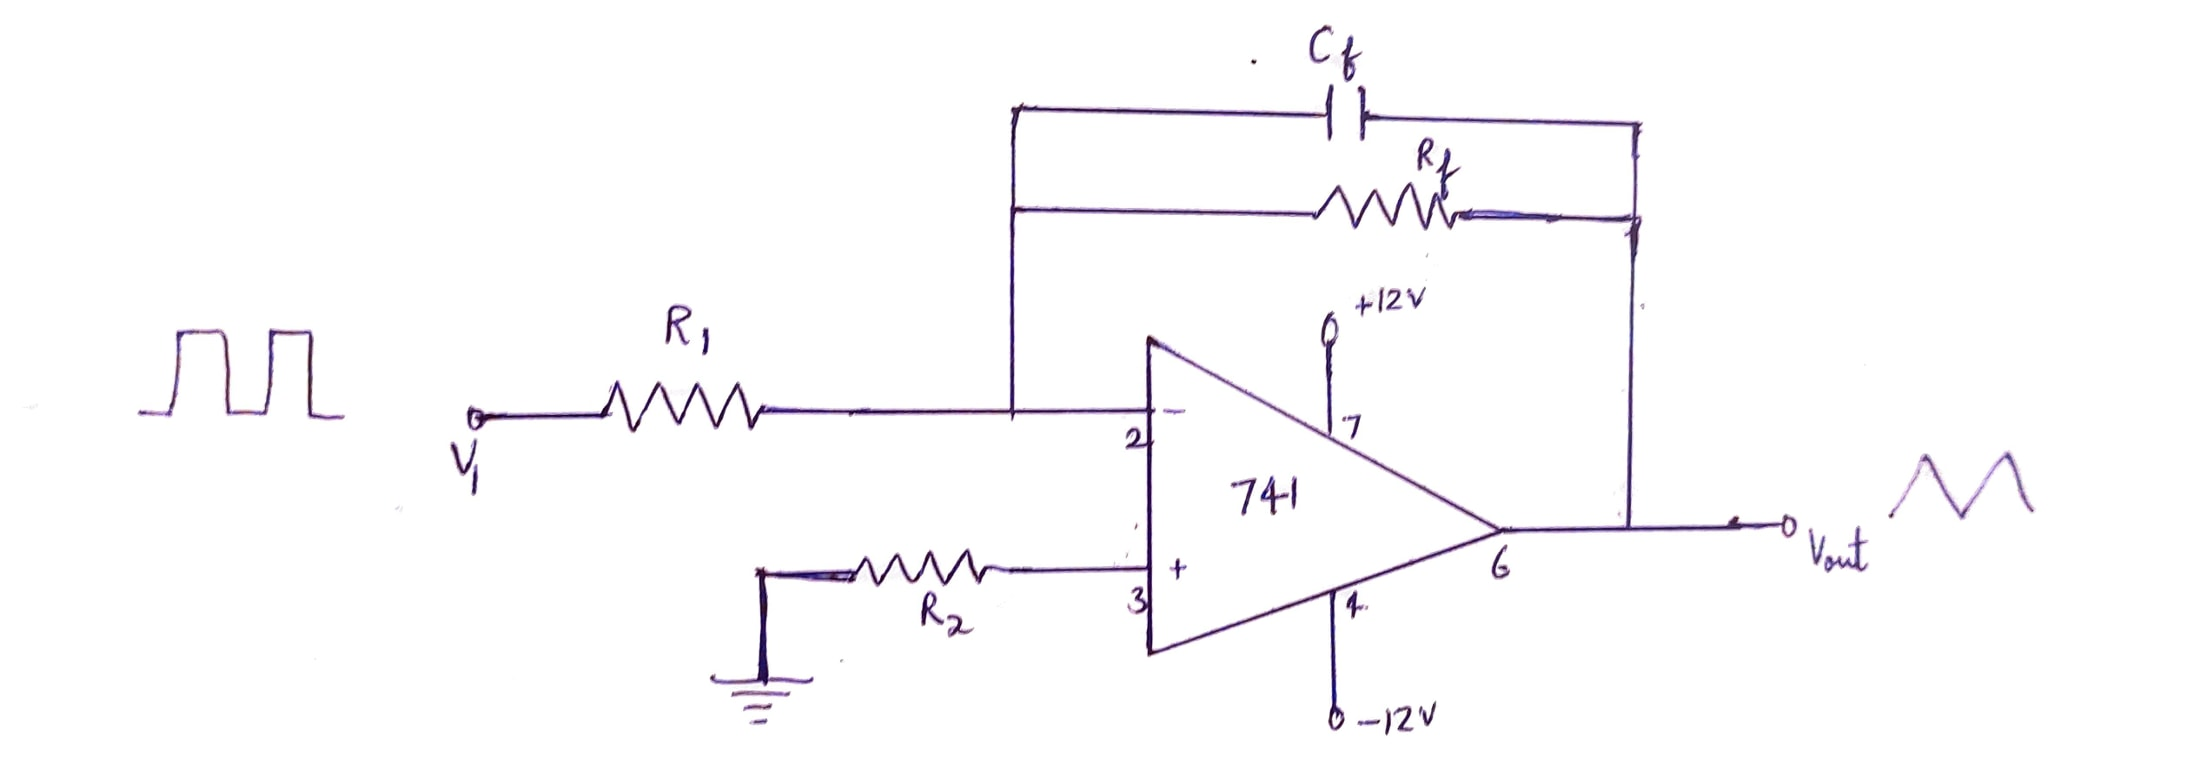
\includegraphics[scale = 0.21]{Documents/intcir.jpg}
\end{center}
\begin{center}
    \textbf{Integrator Amplifier}
\end{center}
\noindent The working of the amplifier can be understood with the help of knowledge of working of RC network circuits. If a constantly varying input signal (an AC signal using a functional generator) is given to the integrator amplifier then the capacitor will charge and discharge in response to changes in the input signal. The resistor $R_2$ is known as the offset minimizing resistor which reduces output
offset voltage due to input bias current. 
\noindent The ideal output voltage for an integrator amplifier is given by
\begin{center}
    $V_{out} = -\dfrac{1}{RC} \int V_{in} dt = - \dfrac{1}{j \omega RC}V_{in}$
\end{center}
\par
\noindent Note that the minus sign indicates a phase shift of $\pi$ radians because the input signal is connected to the inverting input terminal of the operational amplifier. 
\newline
\begin{center}
    \textbf{\large Active Low Pass Filter}
\end{center}
\noindent If the input signal to an Integrator Amplifier is a \emph{sine wave}, we can operate it as a \textbf{\emph{Active Low Pass Filter}}, which will let pass low frequency signals and attenuate the signals beyond a certain frequency. This frequency is known as the \textbf{\emph{Cut-off Frequency}}. The large resistor across the capacitor gives the circuit the characteristics of an inverting amplifier with finite closed-loop gain at low frequencies, while acting as an integrator at high frequencies.
\begin{center}
    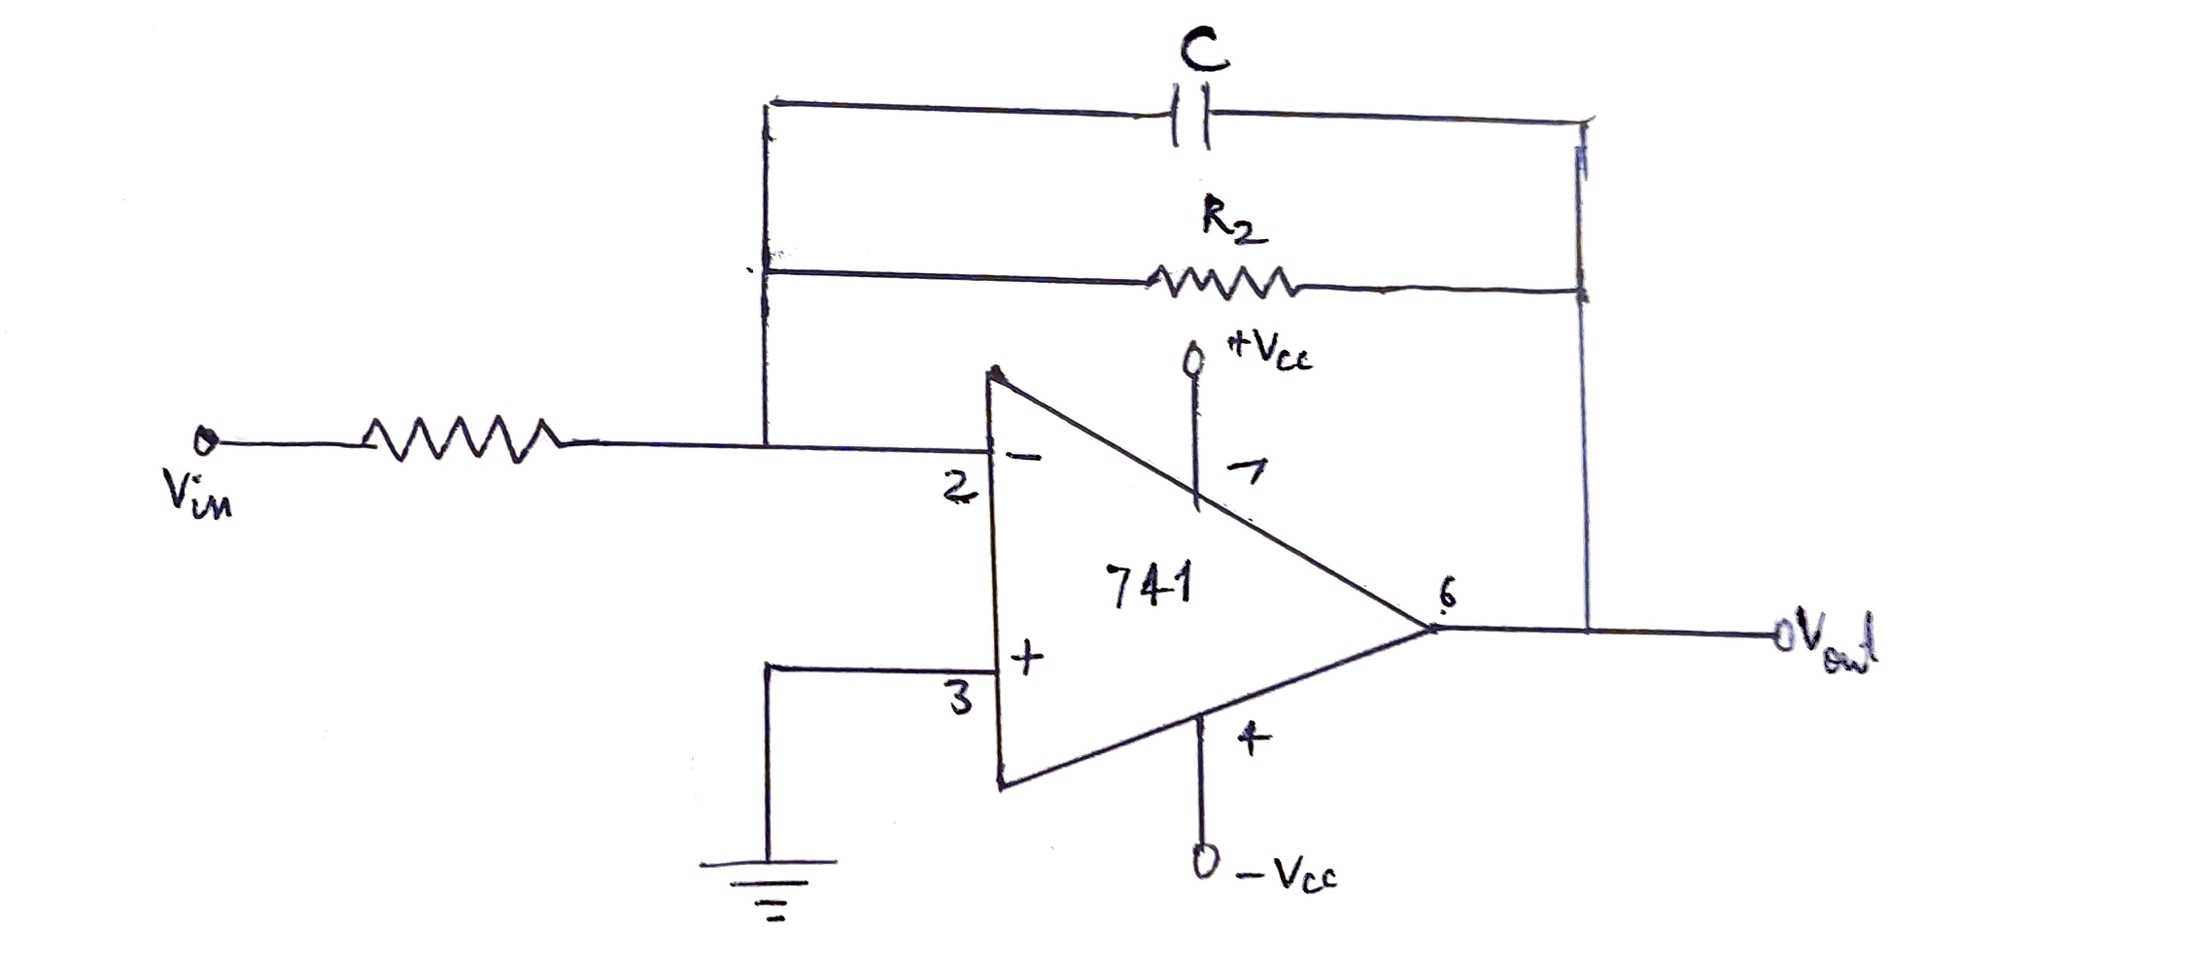
\includegraphics[scale = 0.15]{Documents/filter.jpg}
\end{center}
\begin{center}
    \textbf{First Order Active Low Pass Filter}
\end{center}
The cut-off frequency is given by
\begin{center}
    $f_c = \dfrac{1}{2 \pi R_2 C}$
\end{center}
The gain of an active low pass filter is given by
\begin{center}
    $A = - \dfrac{(R_2 || X_C)}{R_1}$ 
\end{center}
where $X_C = \dfrac{1}{2 \pi f C}$ is the impedance of the capacitor $C$ and $f$ is the frequency of the input signal 
\par
\begin{center}
    \textbf{\large Differentiator Amplifier}
\end{center}
\noindent The \textbf{\emph{Differentiator Amplifier}} is a configuration of an RC-coupled Op-Amp circuit which performs the mathematical operation of \emph{differentiation}. Its working is exactly opposite to that of an Integrator Amplifier. It produces a voltage output which
is proportional to the rate of change of the input voltage and the current flowing through the
capacitor. In other words, the faster or larger the change to the input voltage signal, the greater
the input current, the greater will be the output voltage change.
\par
\noindent The circuit diagram for the differentiator amplifier is as follows:
\begin{center}
    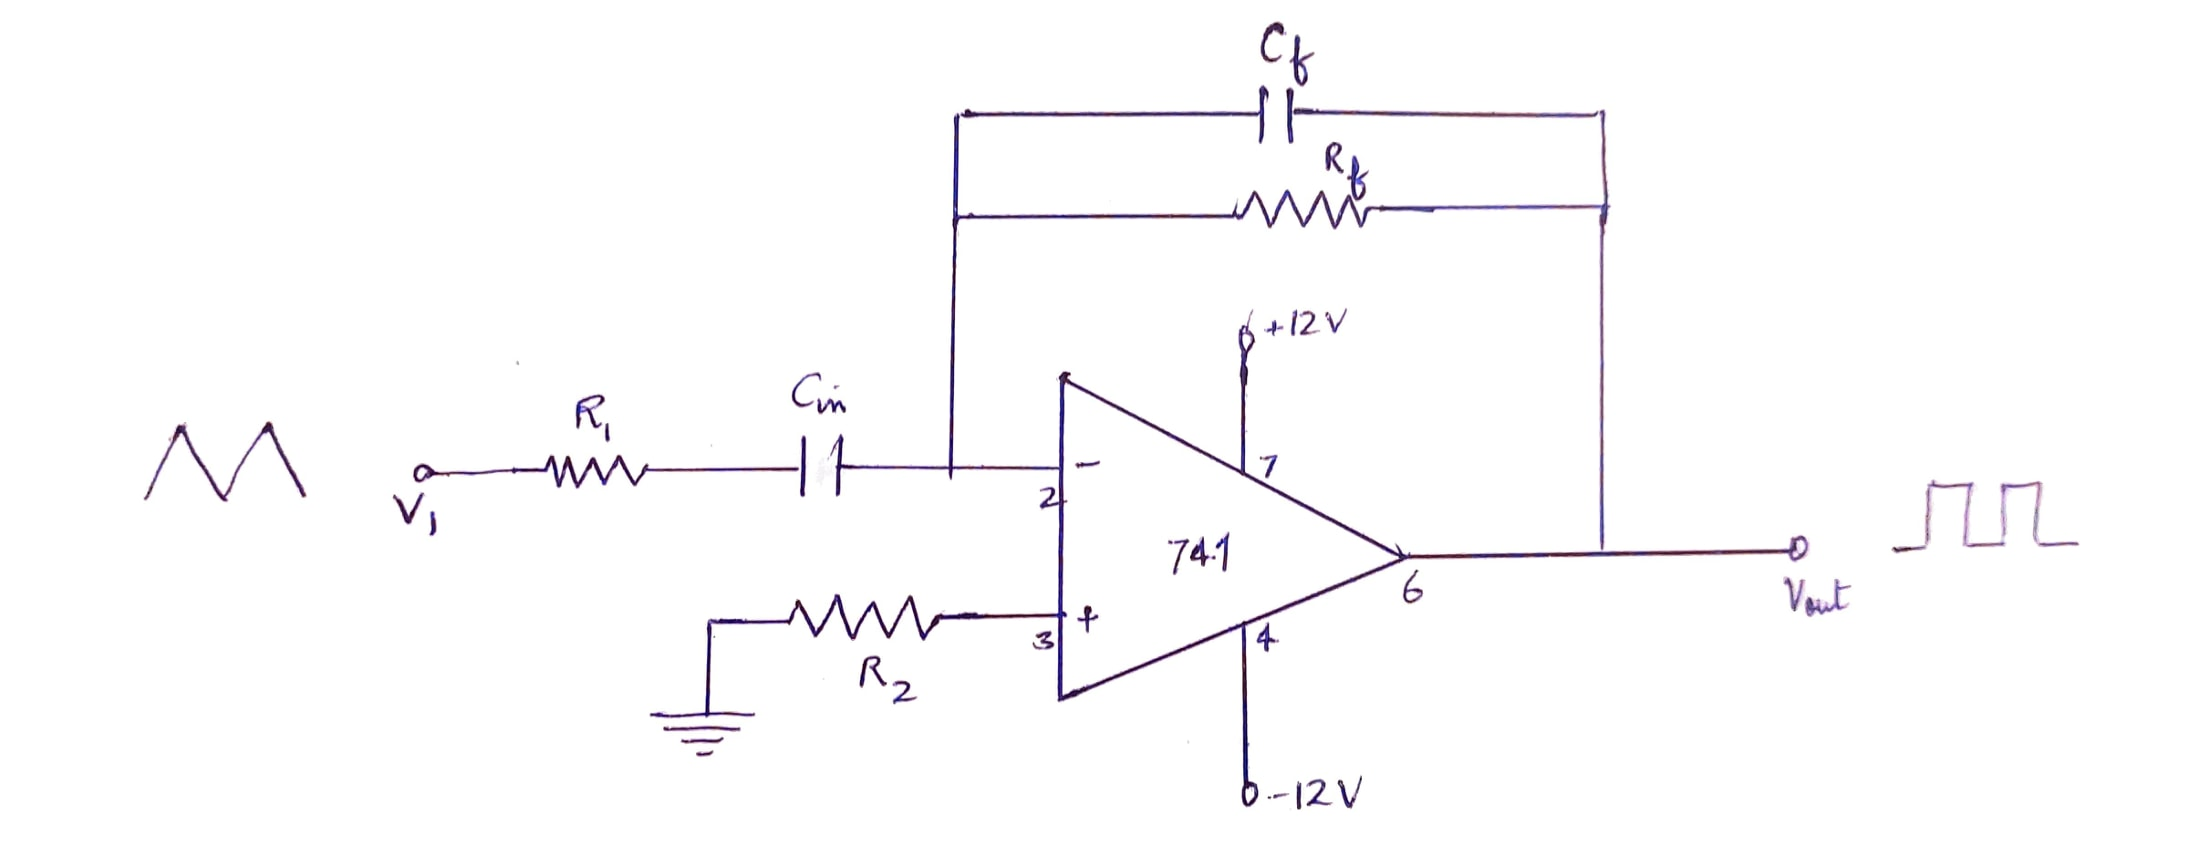
\includegraphics[scale = 0.2]{Documents/diffcir.jpg}
\end{center}
\begin{center}
    \textbf{Differentiator Amplifier}
\end{center}
\noindent The ideal output voltage for an differentiator amplifier is given by
\begin{center}
    $V_{out} = - R_f C \dfrac{dV_{in}}{dt}$
\end{center}
\noindent Again, the minus sign appears due to the existence of the phase difference of $\pi$ radians. The role of the resistor $R_2$ is also same to that of its role in the integrator amplifier.
\section{Observations}
\begin{center}
    \textbf{For Integrator Amplifier}
\end{center}
\begin{center}
    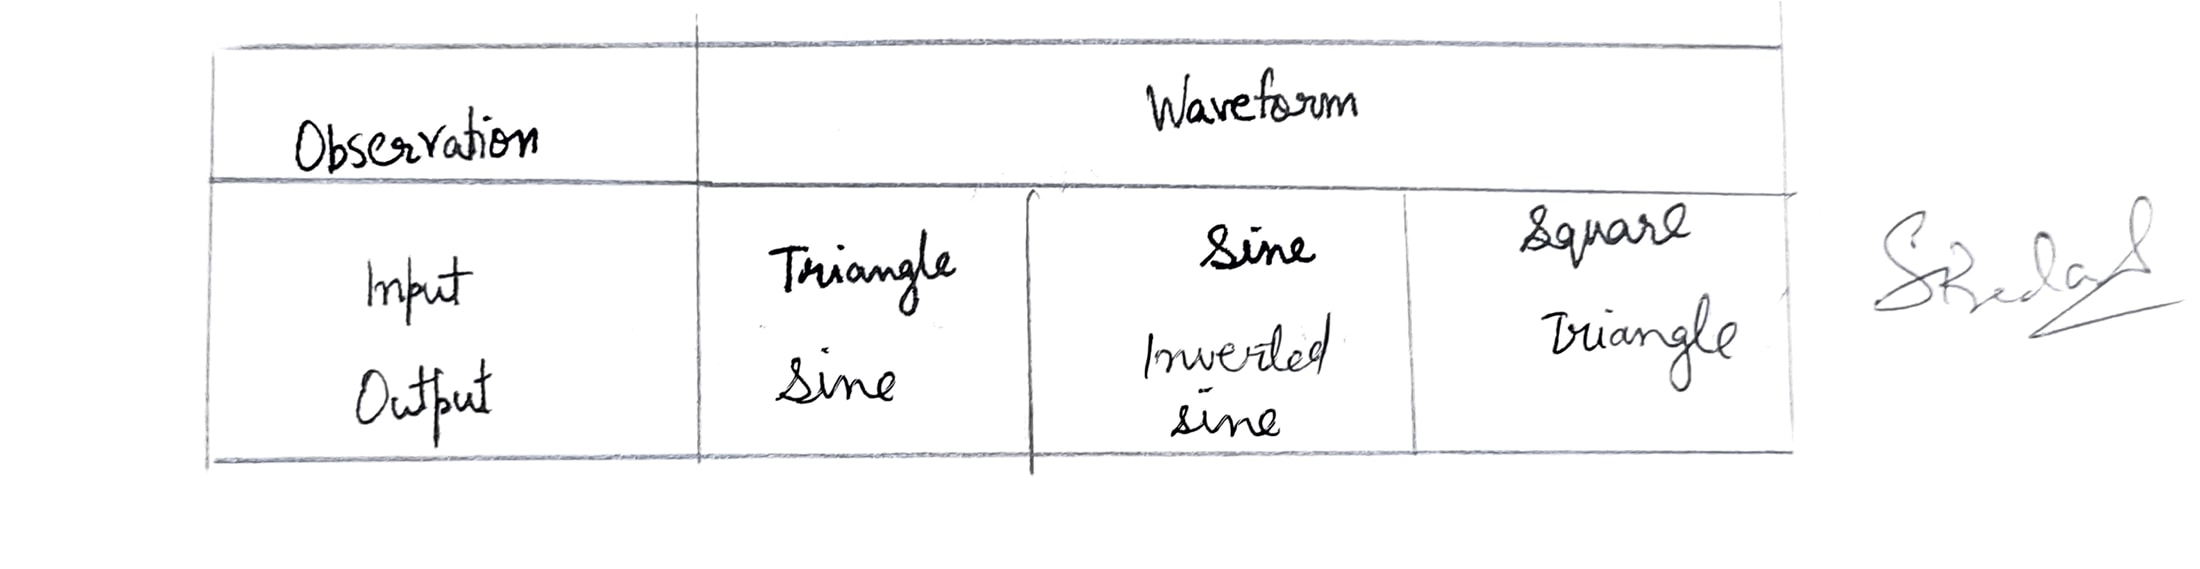
\includegraphics[scale = 0.15]{Documents/int.jpg}
\end{center}
\begin{center}
    \textbf{For Differentiator Amplifier}
\end{center}
\begin{center}
    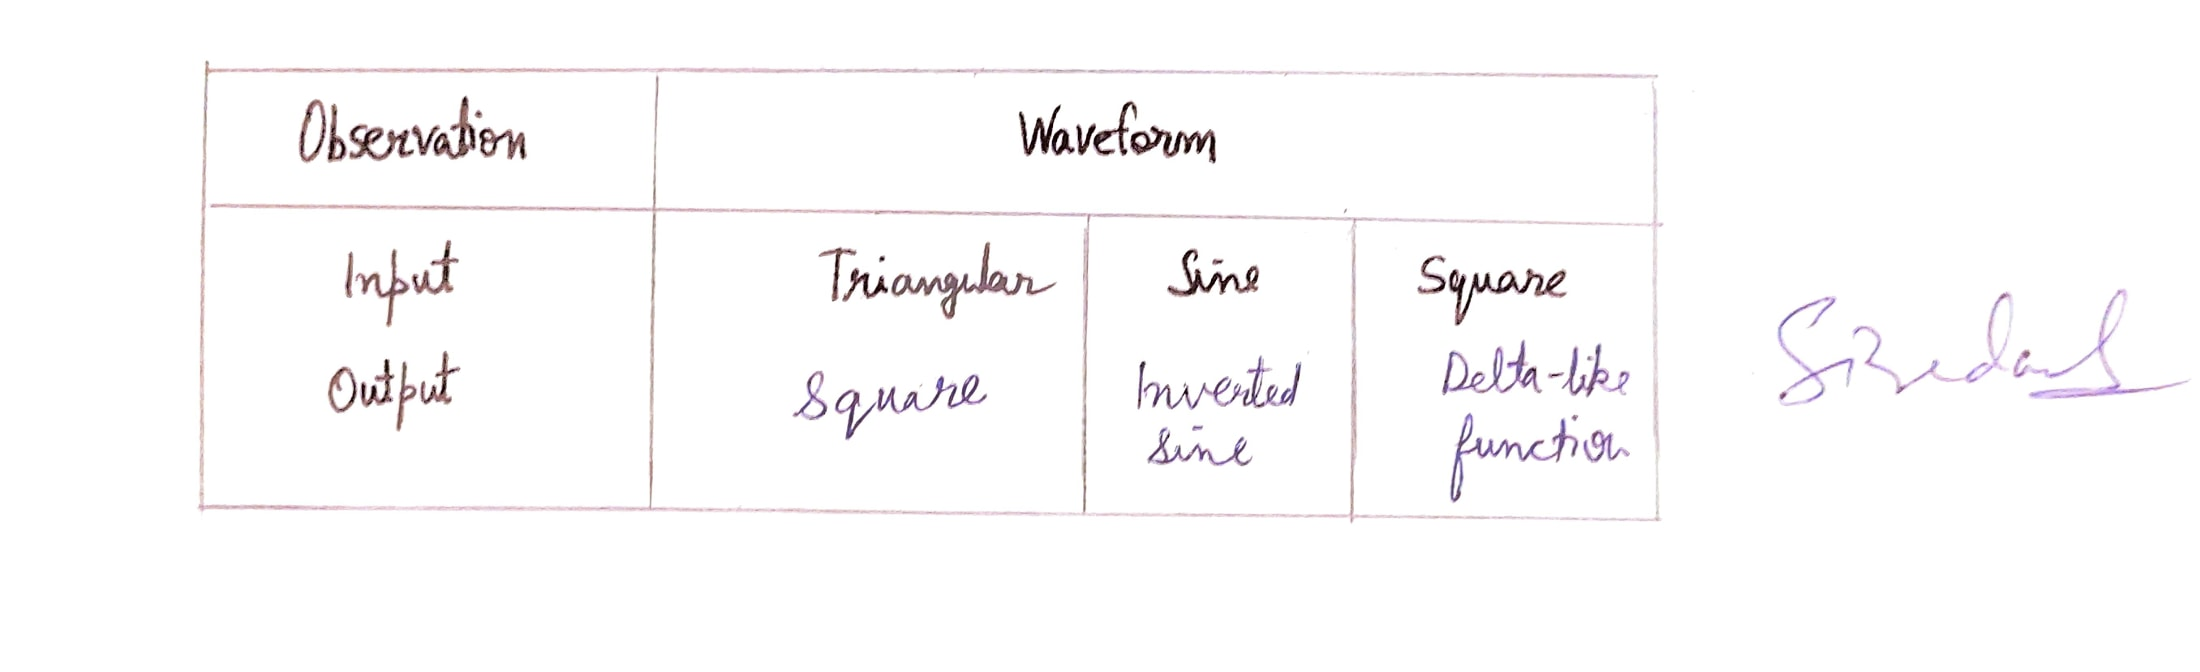
\includegraphics[scale = 0.15]{Documents/diff.jpg}
\end{center}
\begin{center}
    \textbf{Oscilloscope Results for Integrator}
\end{center}
\begin{center}
    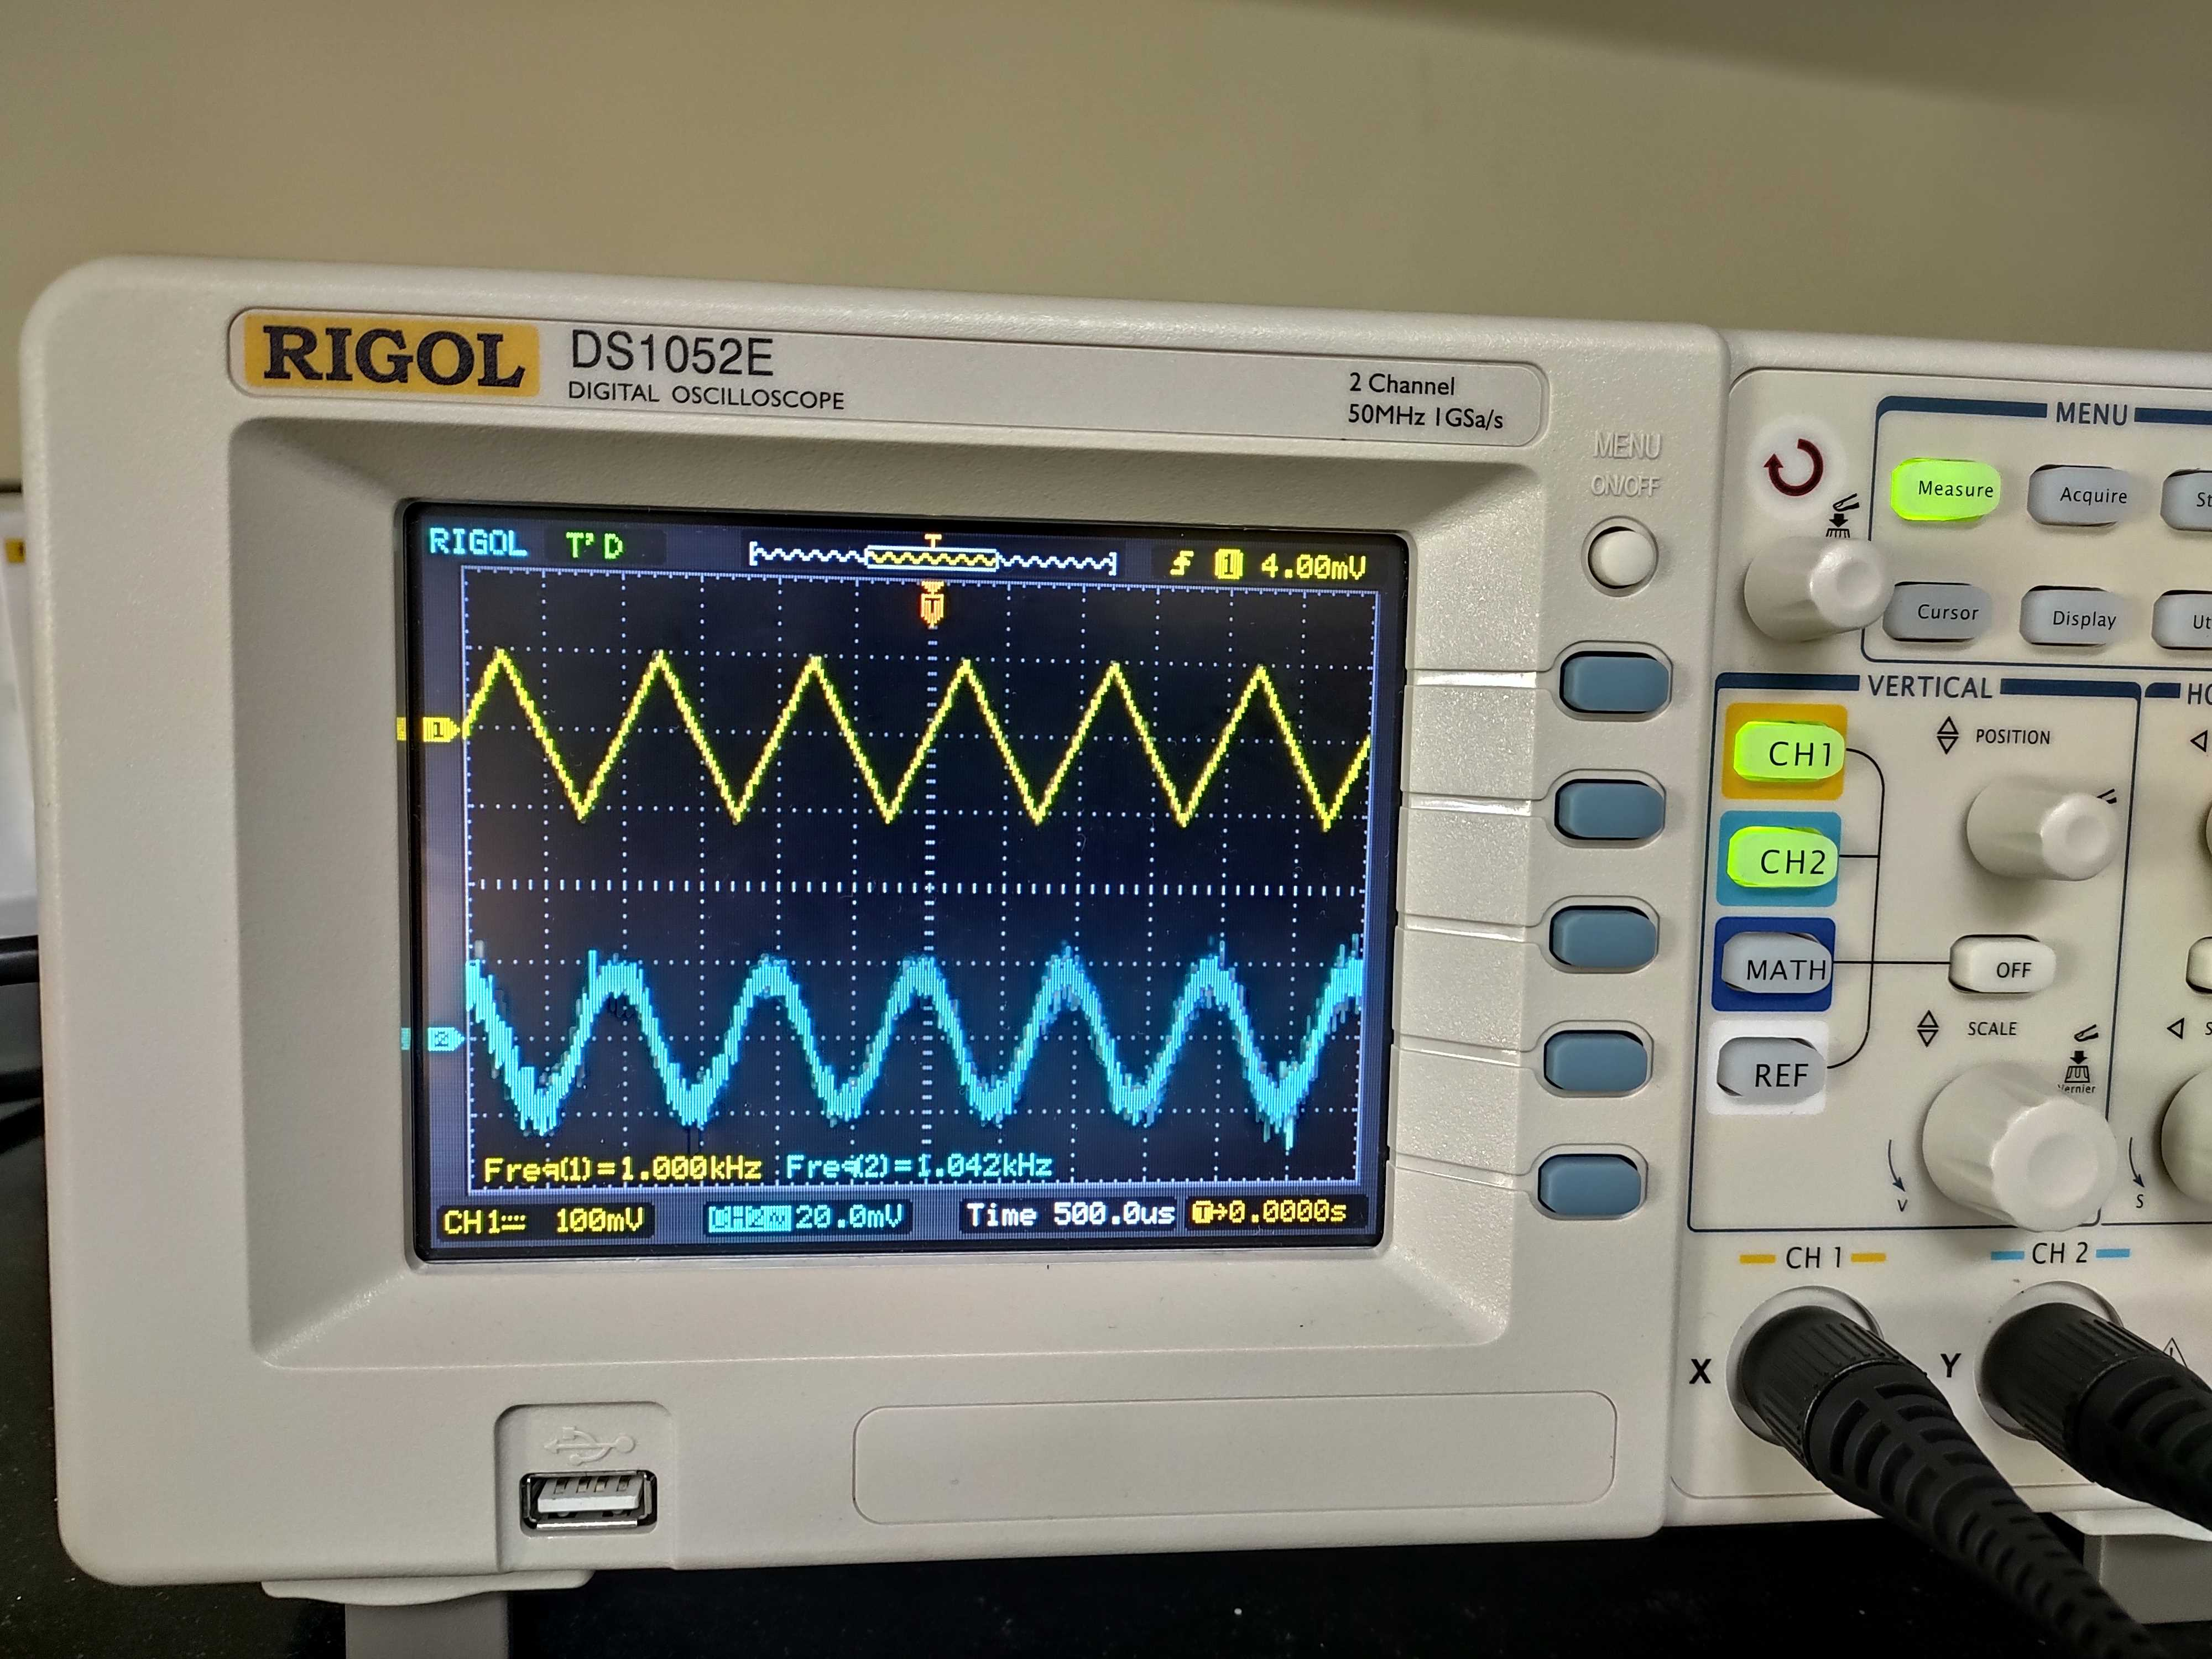
\includegraphics[scale = 0.09]{Documents/Int. Triangle.jpg}
\end{center}
\bigskip
\begin{center}
    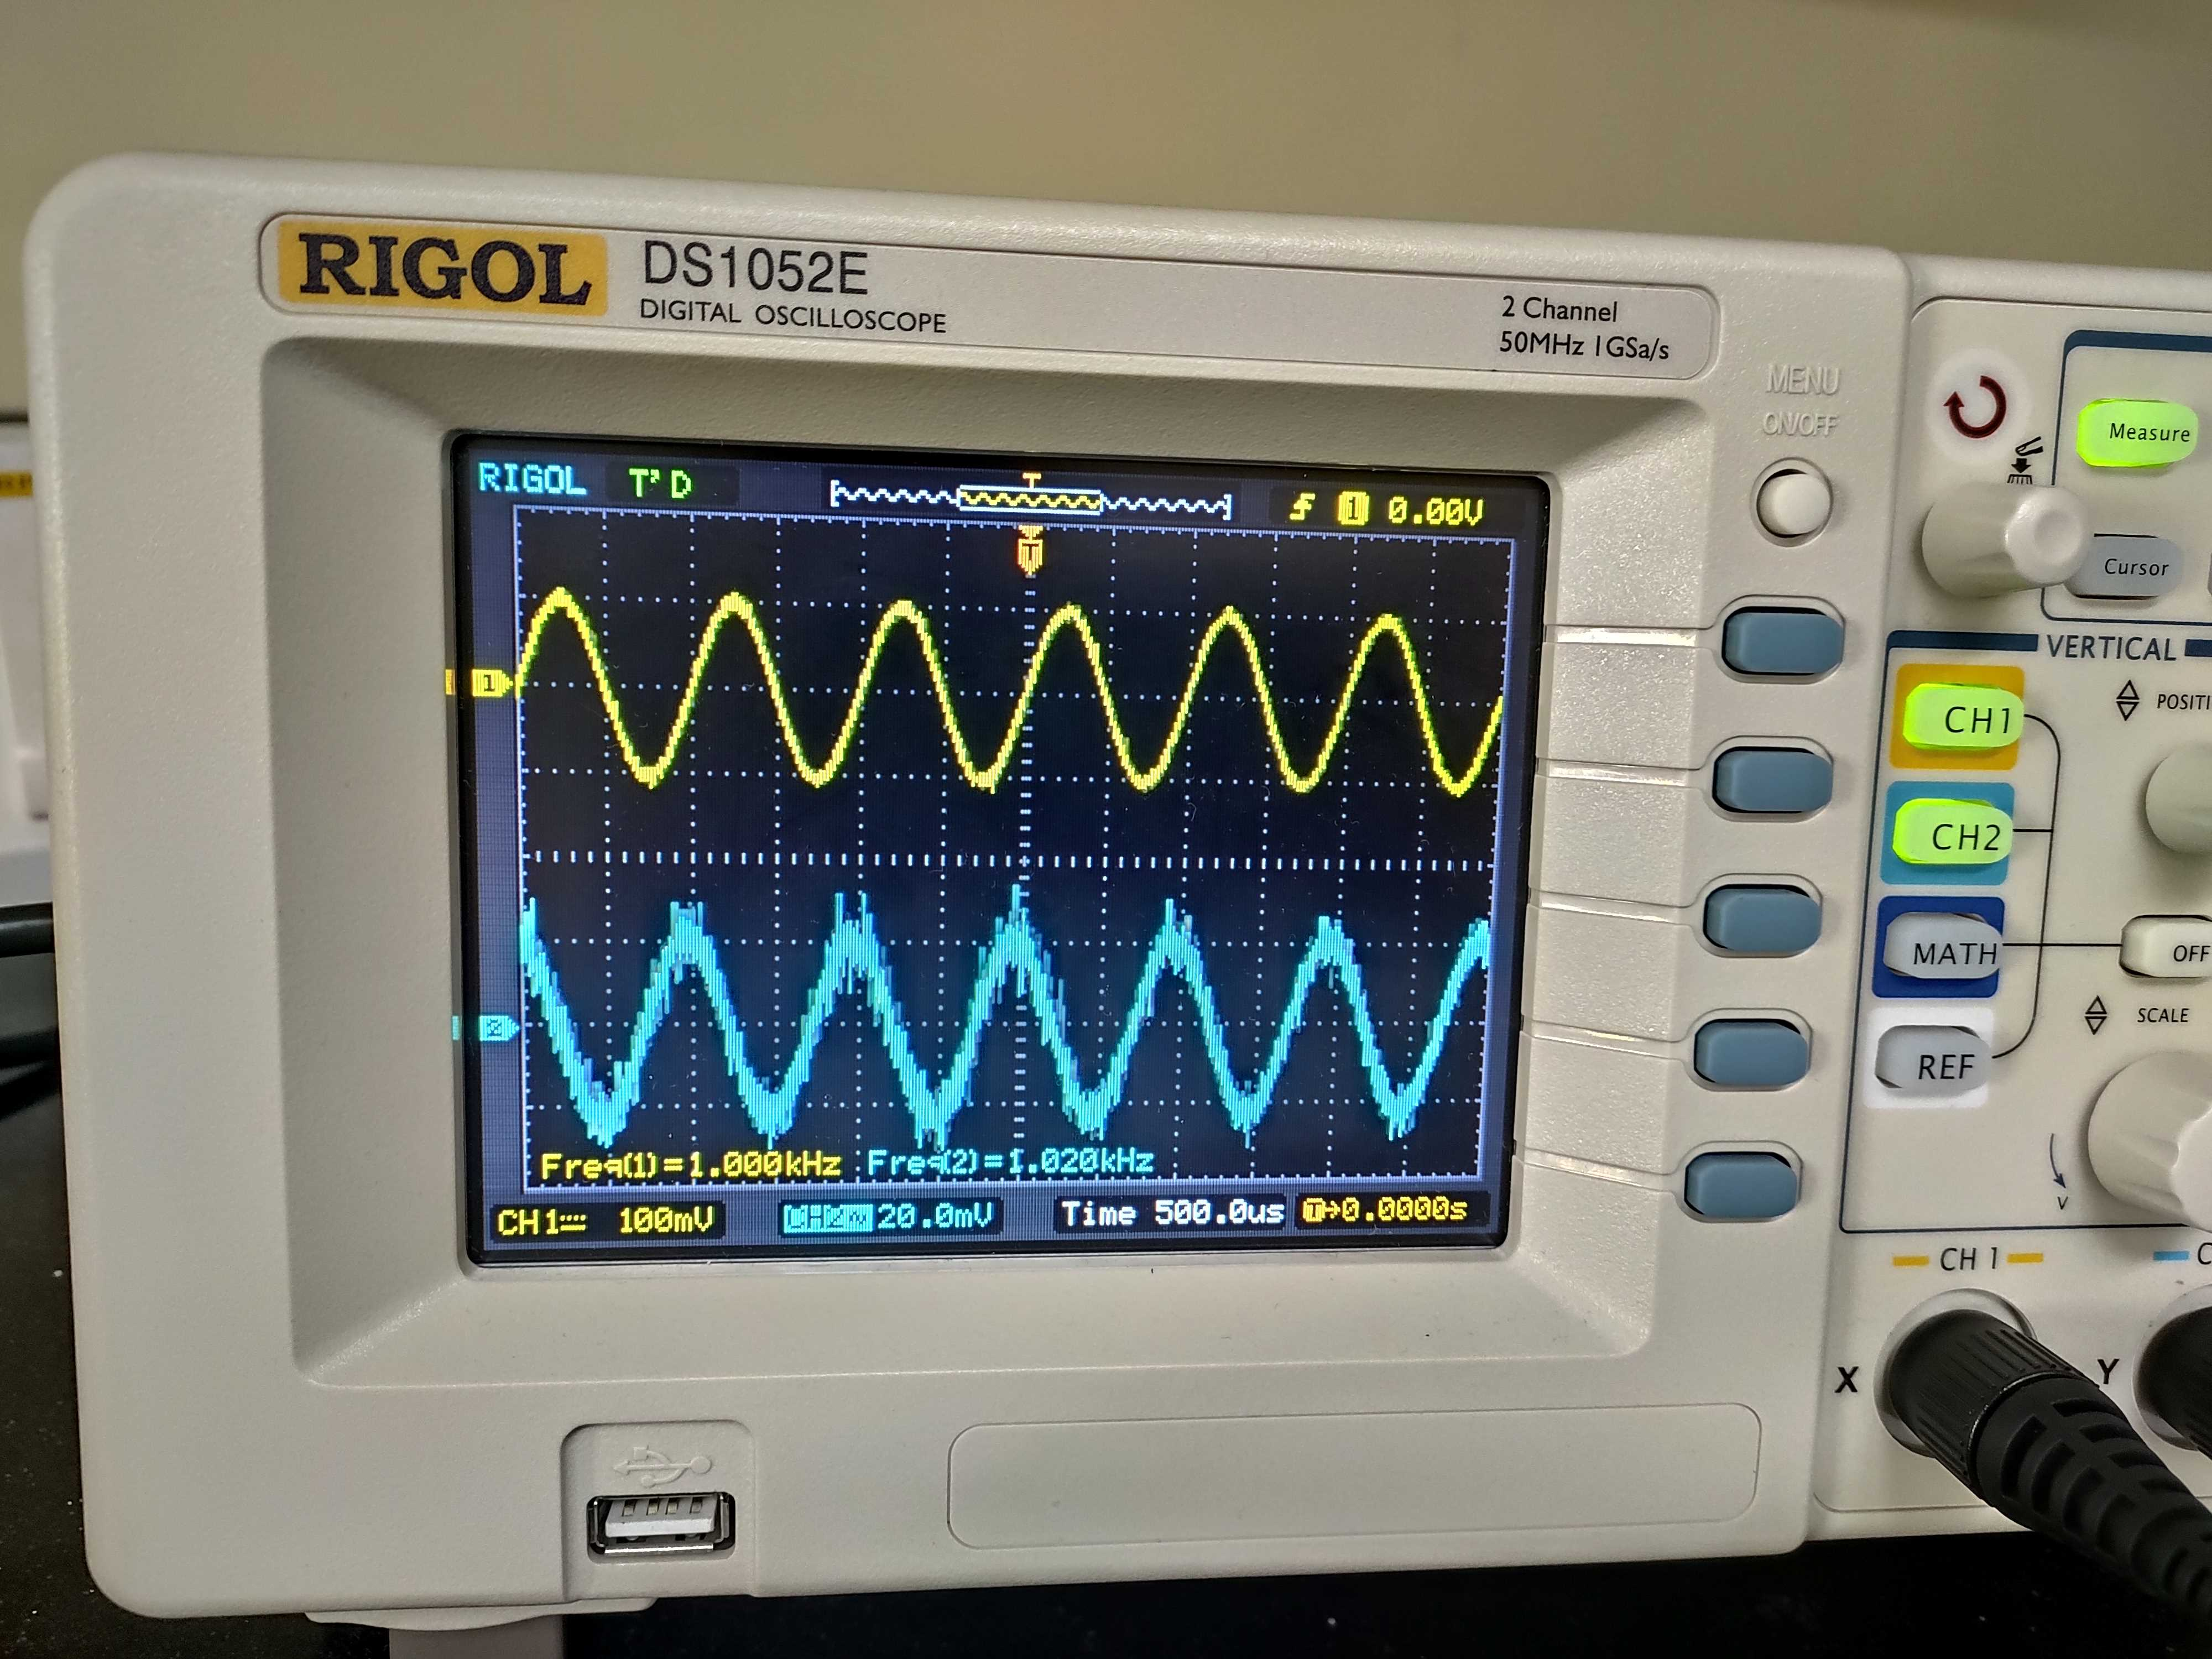
\includegraphics[scale = 0.09]{Documents/Int. Sine.jpg}
\end{center}
\begin{center}
    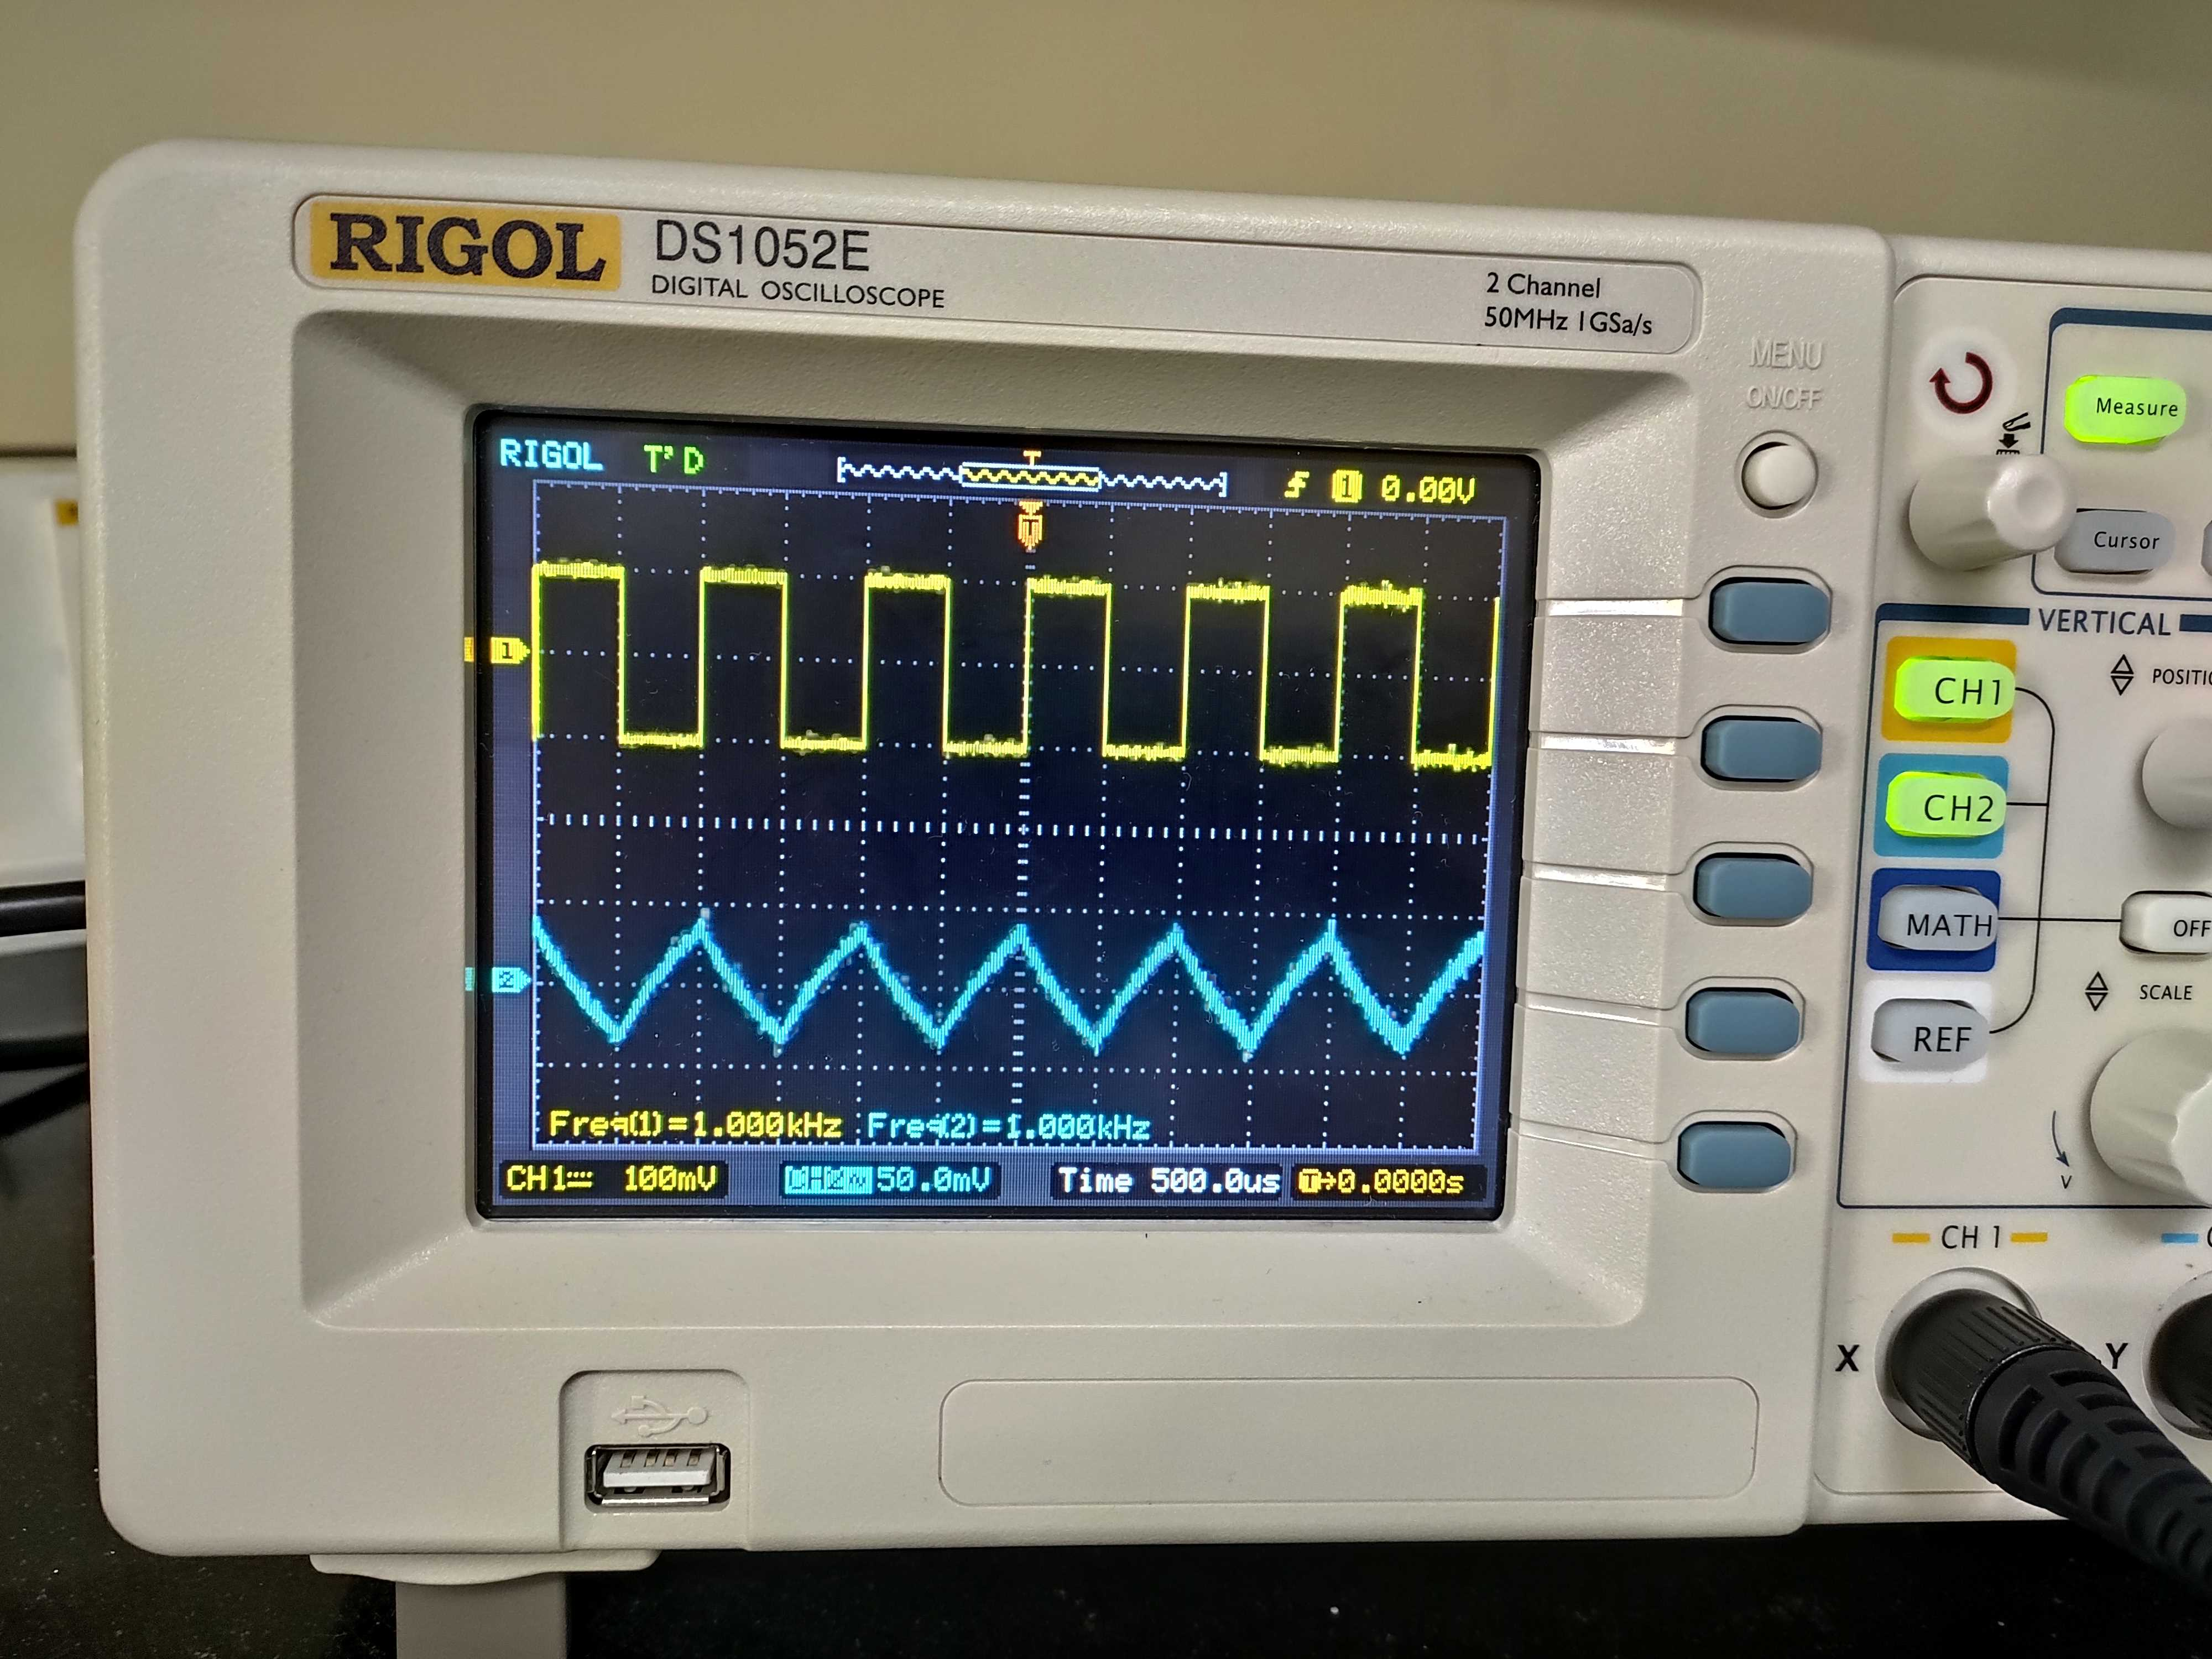
\includegraphics[scale = 0.09]{Documents/Int. Square.jpg}
\end{center}
\bigskip
\begin{center}
    \textbf{Oscilloscope Results for Differentiator}
\end{center}
\begin{center}
    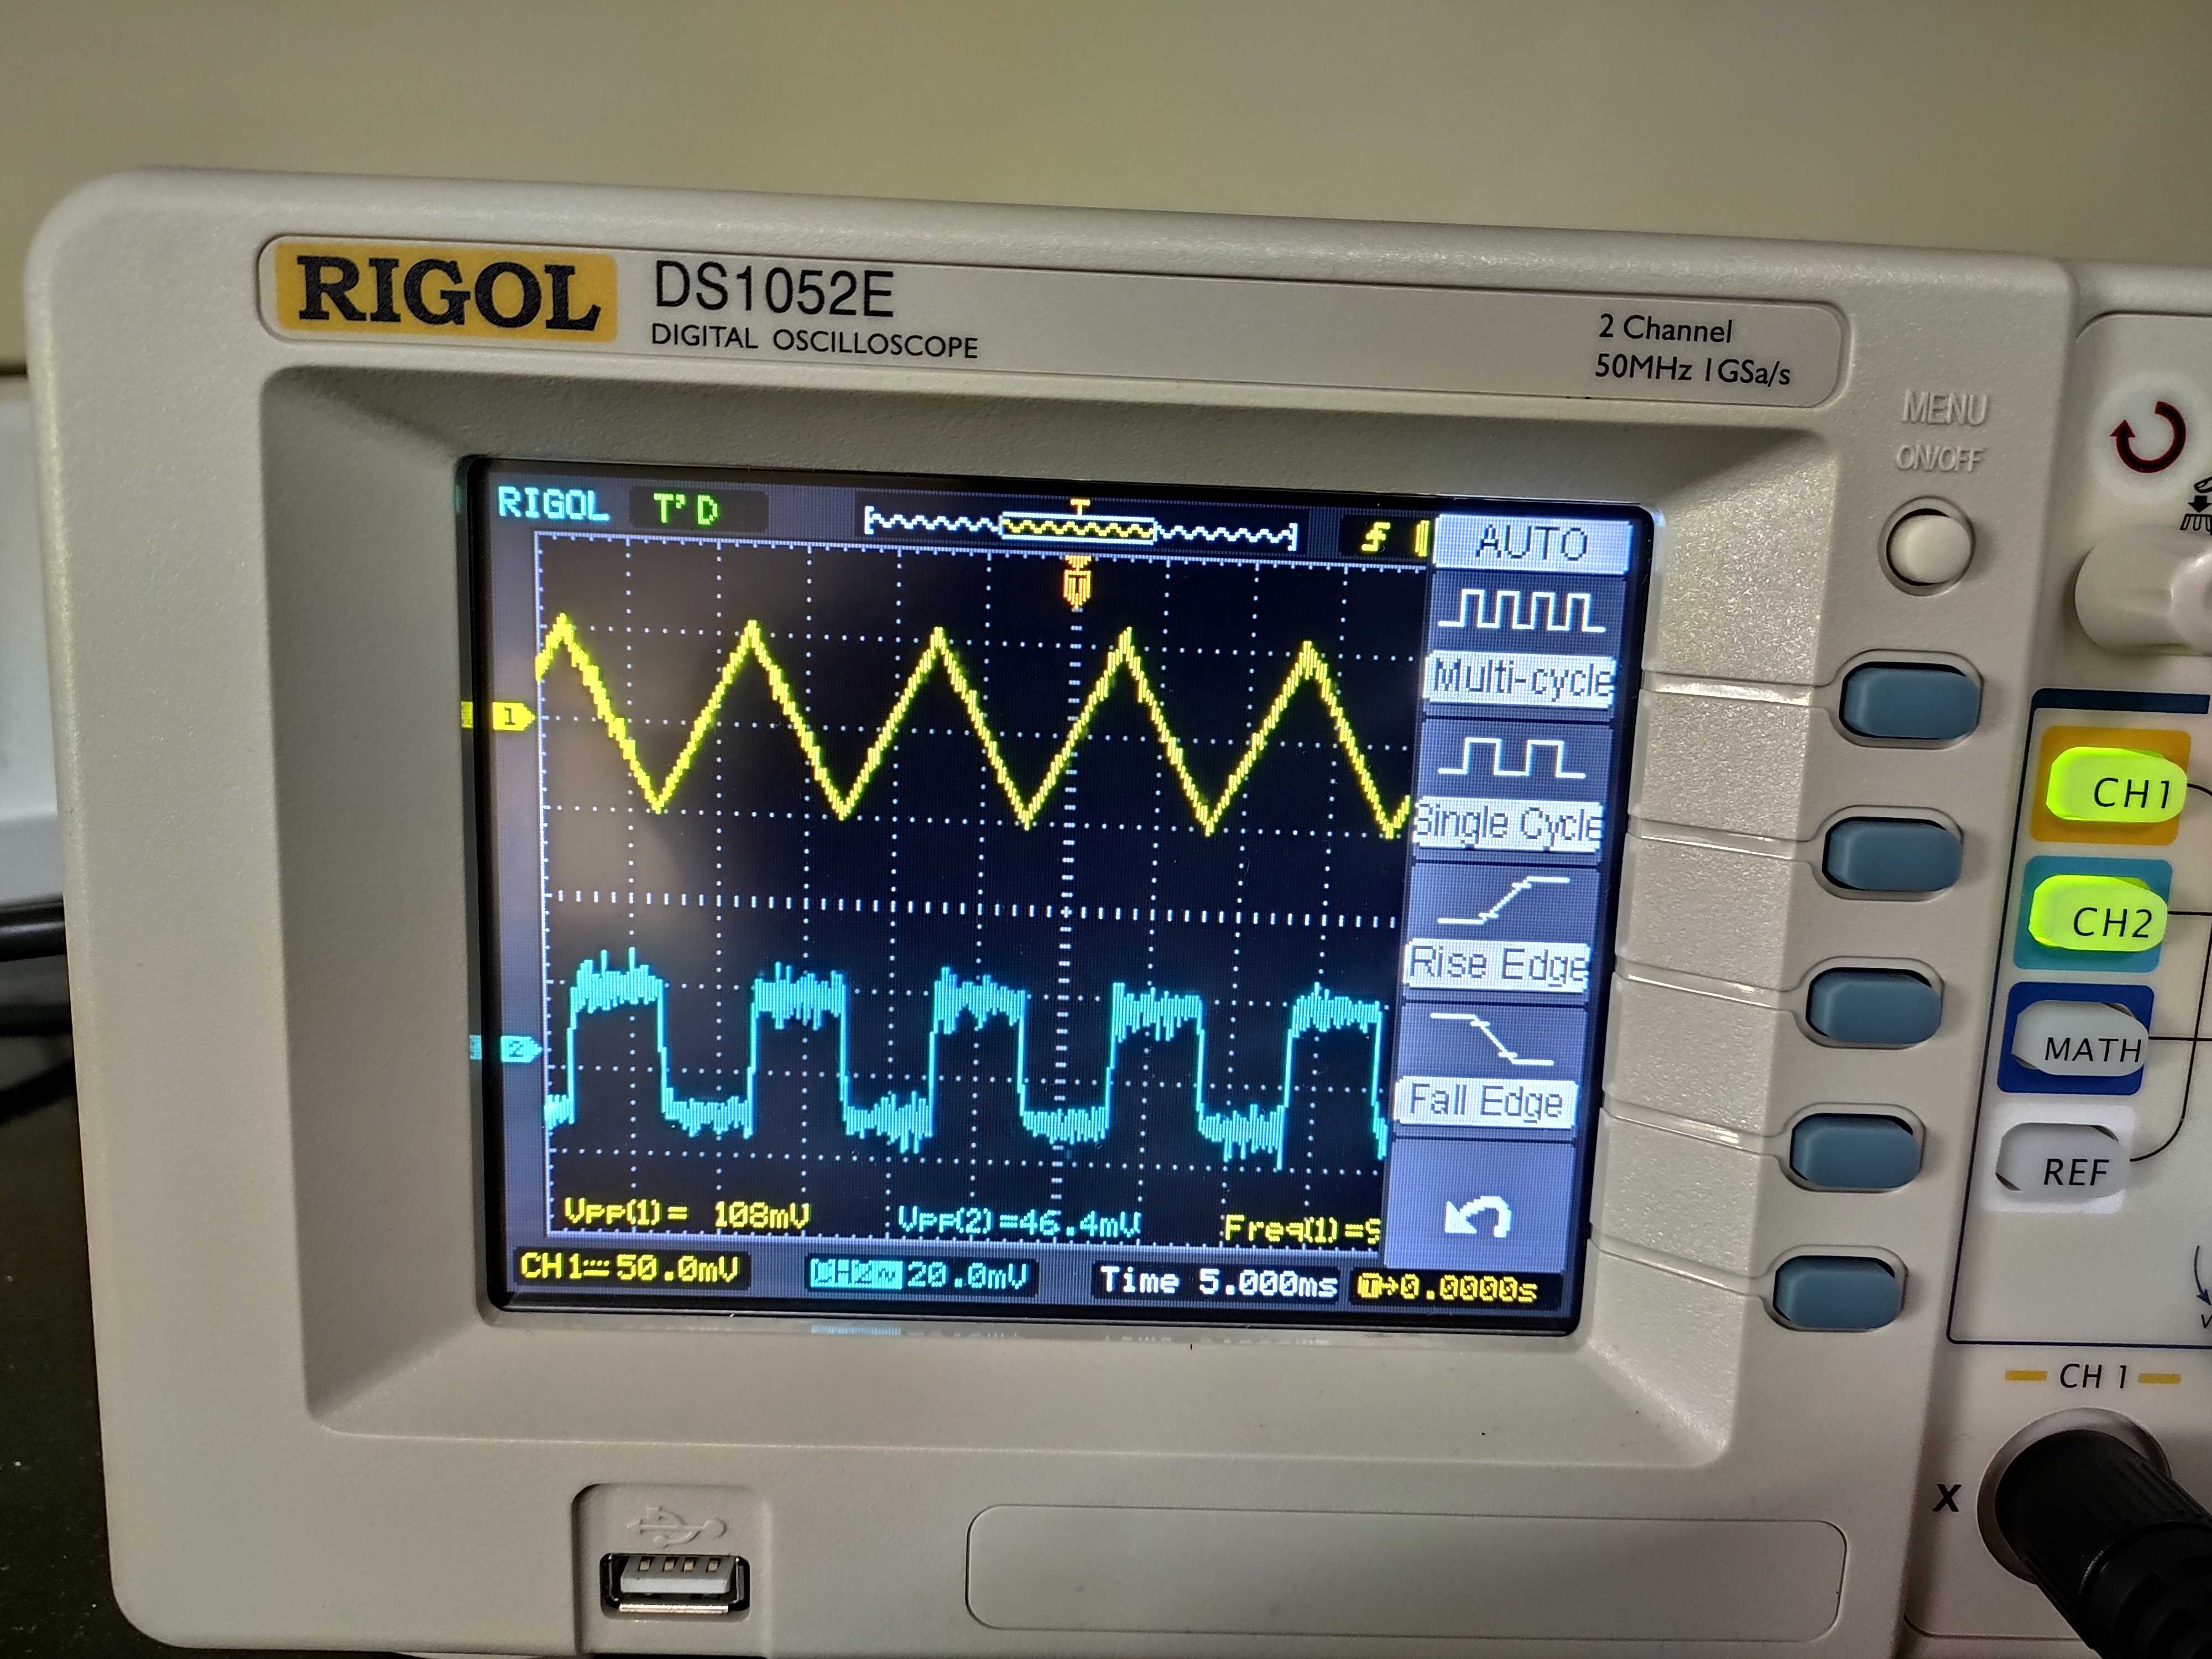
\includegraphics[scale = 0.09]{Documents/Diff. Triangle.jpg}
\end{center}
\begin{center}
    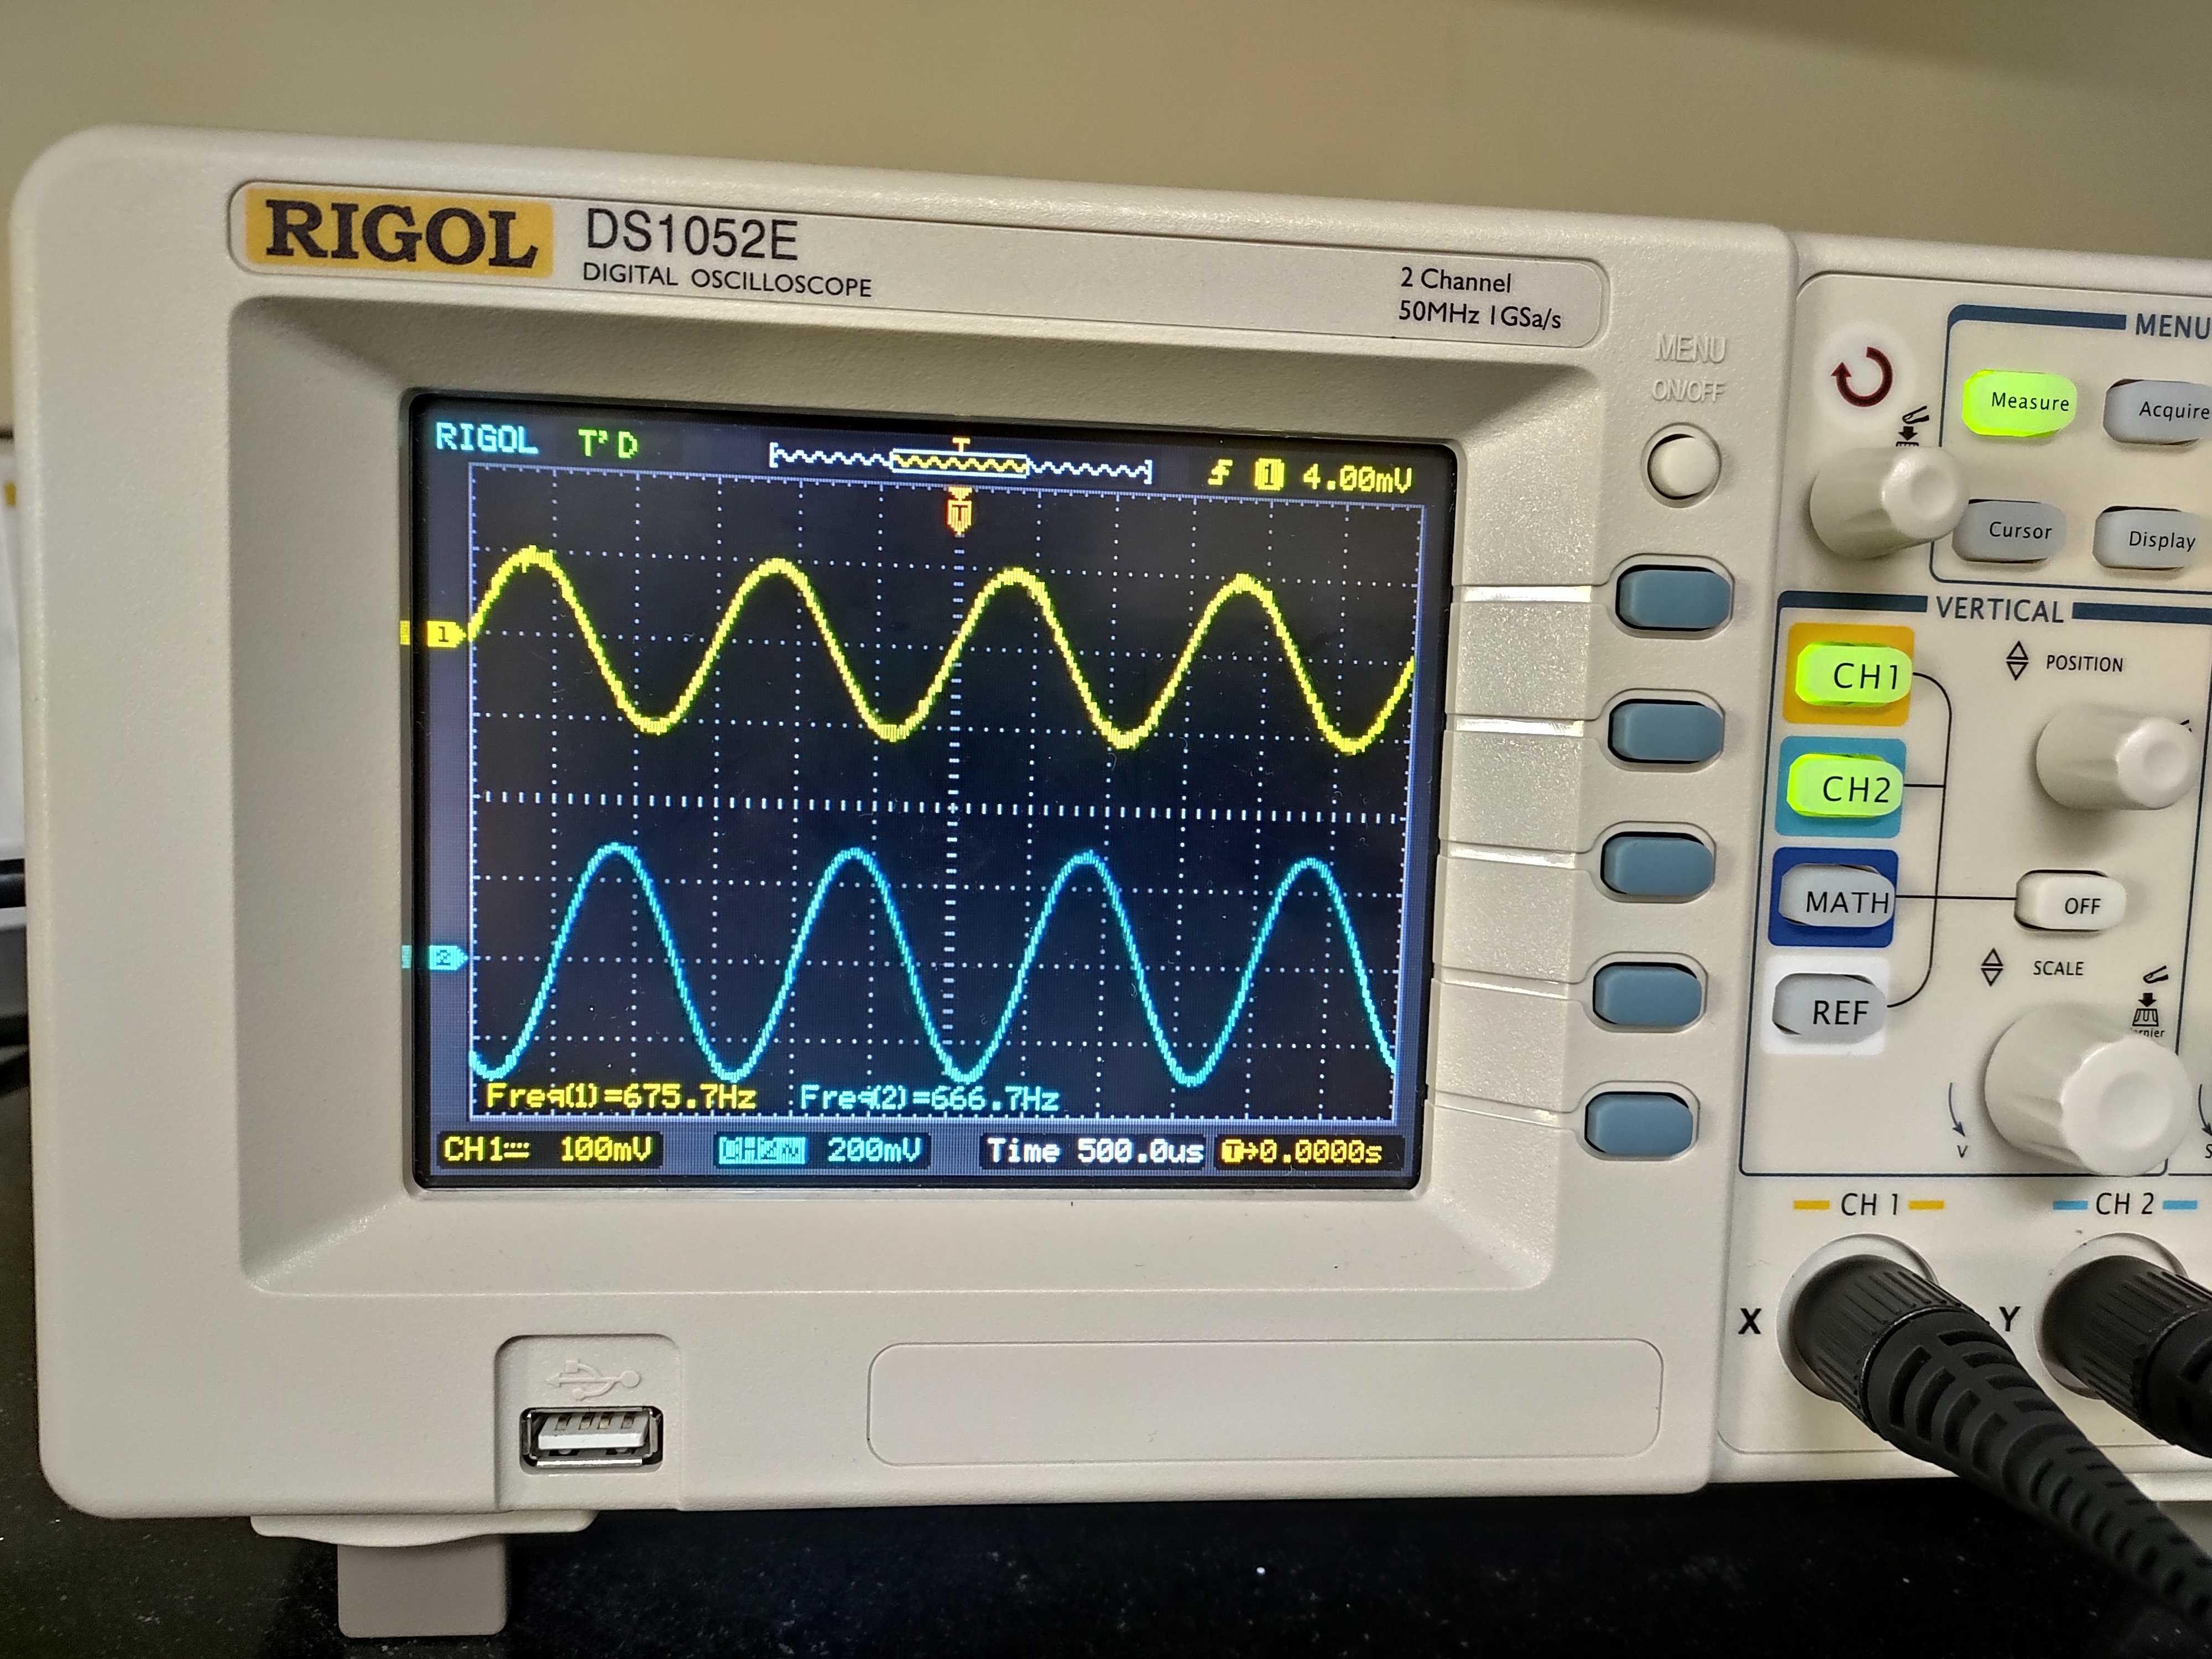
\includegraphics[scale = 0.09]{Documents/Diff. Sine.jpg}
\end{center}
\bigskip
\begin{center}
    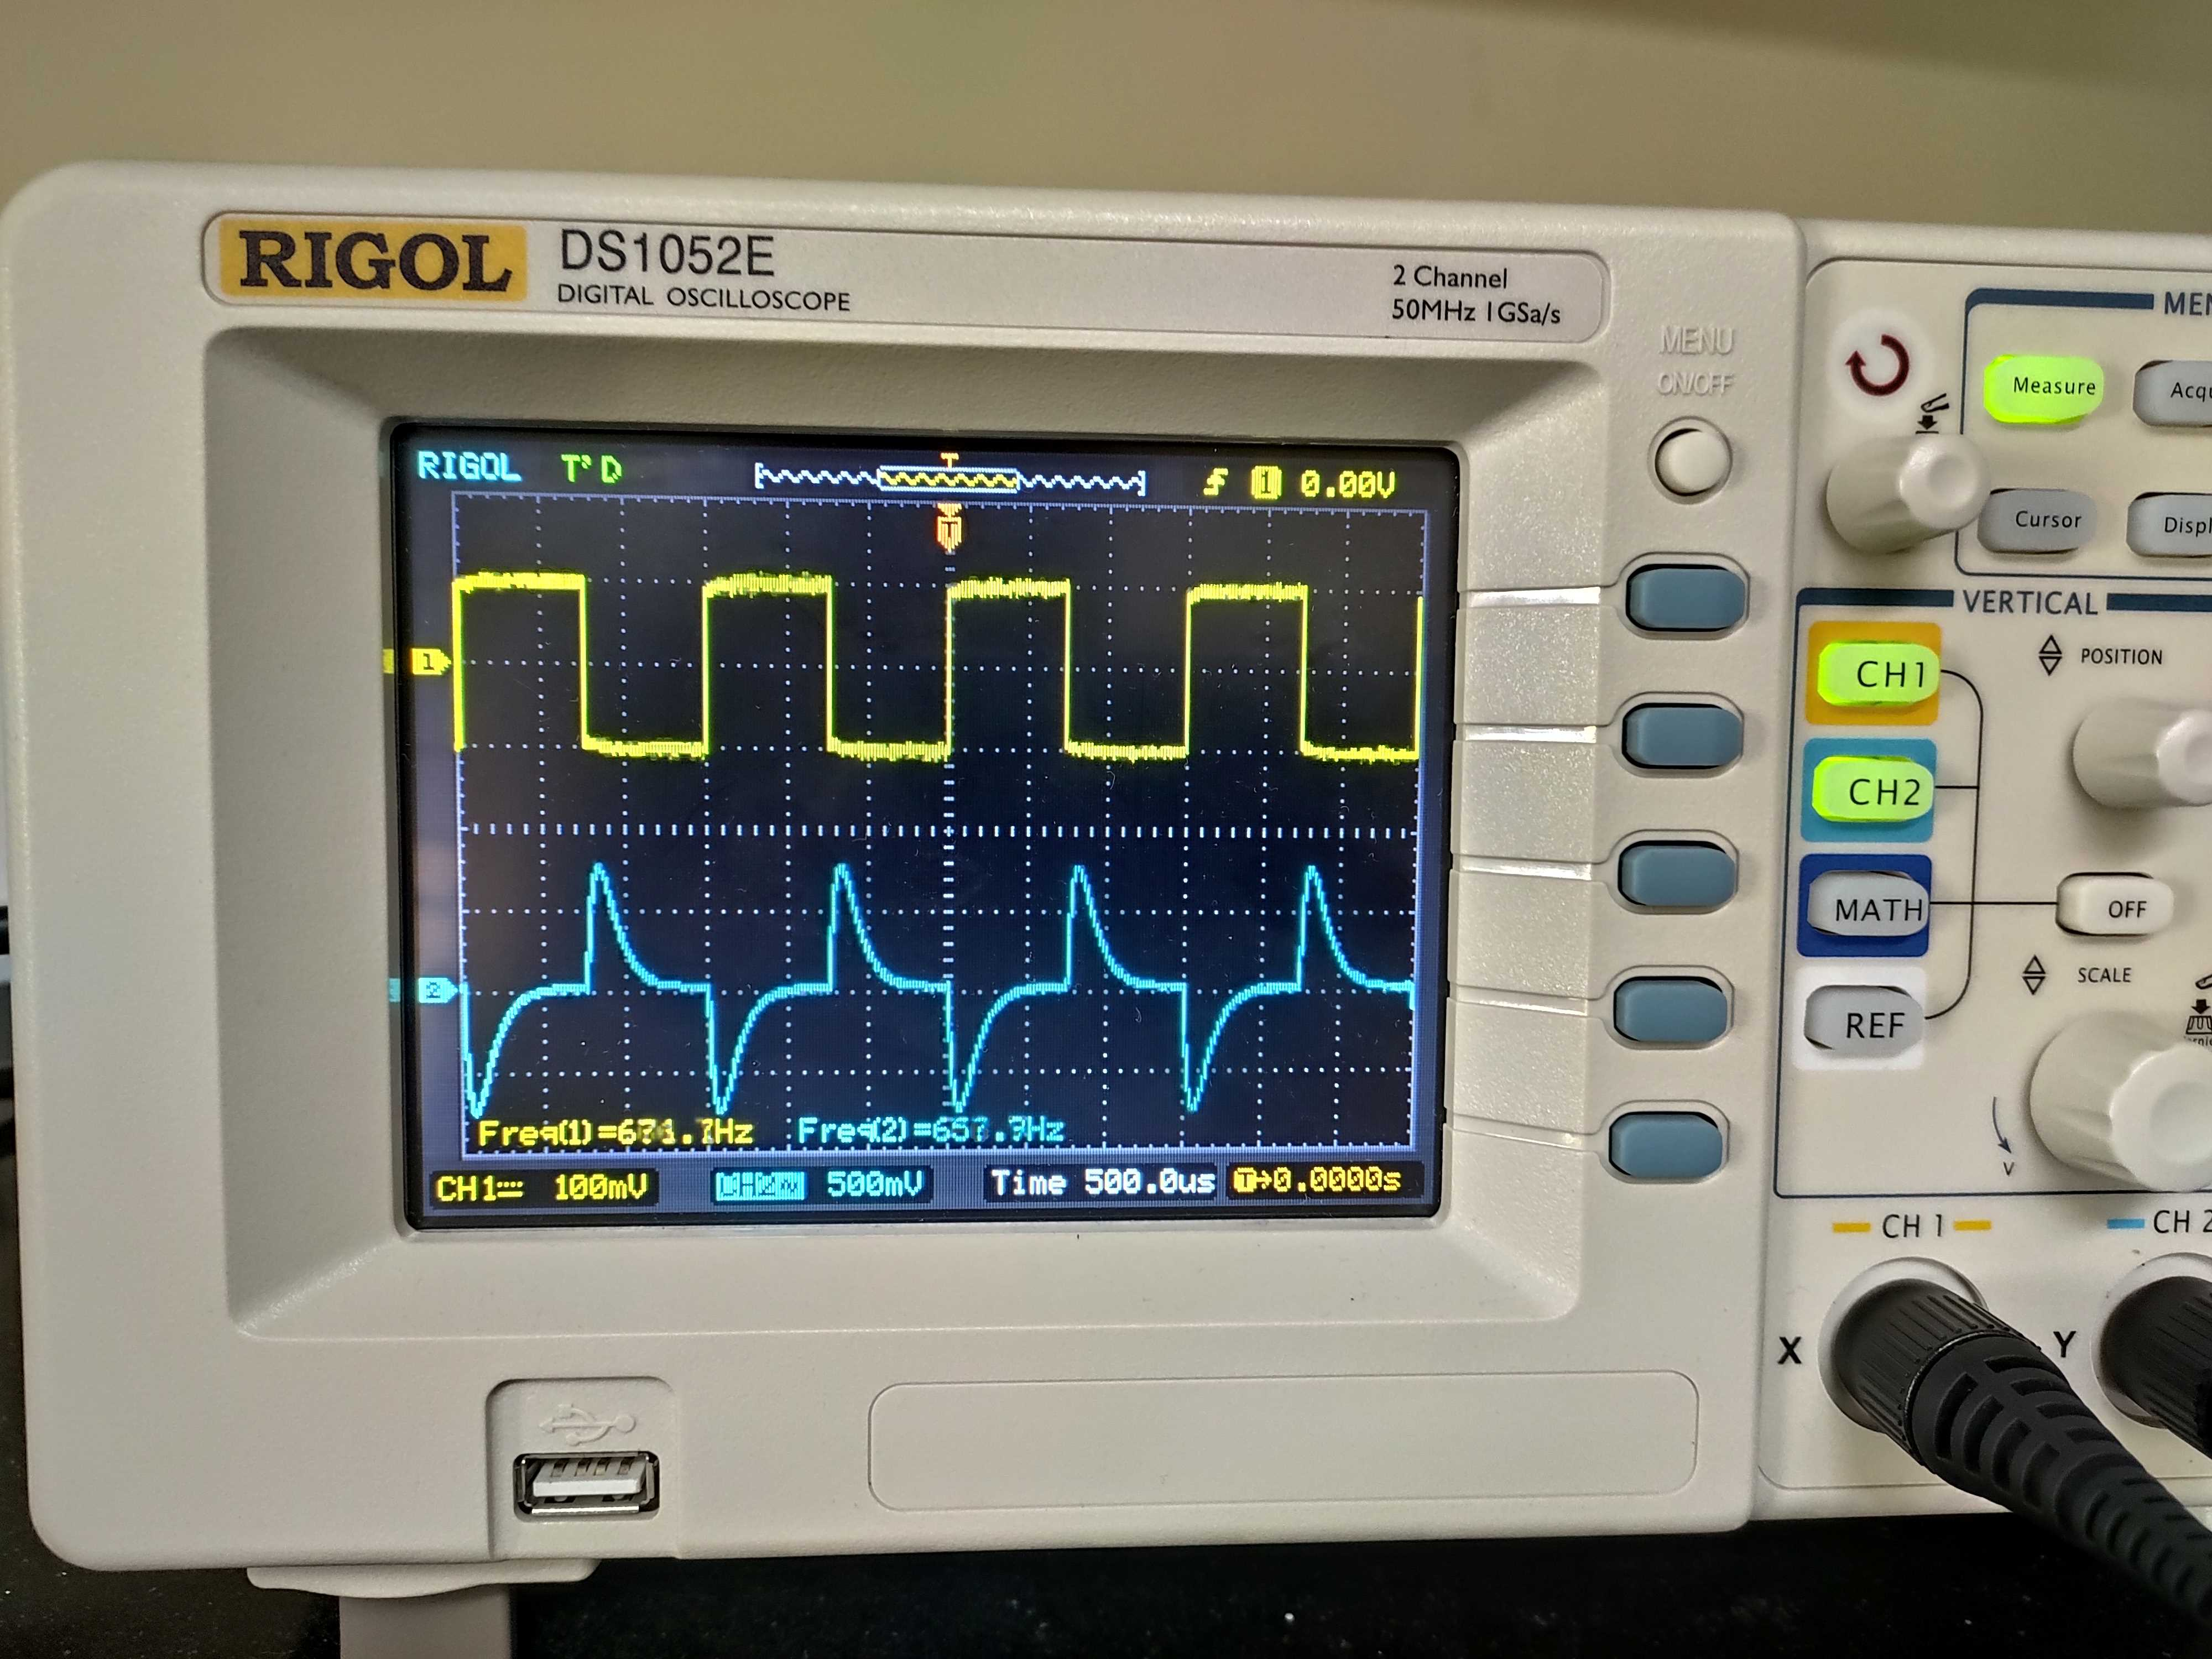
\includegraphics[scale = 0.09]{Documents/Diff. Square.jpg}
\end{center}
\clearpage
\begin{center}
    \textbf{For Active Low Pass Filter}
\end{center}
$C = \SI{81.0}{n \farad}$; $f_{c} = \dfrac{1}{2 \pi R_2 C} = \SI{197.47}{\hertz}$; $R_1 = \SI{1.015}{k\ohm}$; $R_2 = \SI{9.95}{k\ohm}$; $-\dfrac{R_2}{R_1} = -9.80$.
\begin{center}
    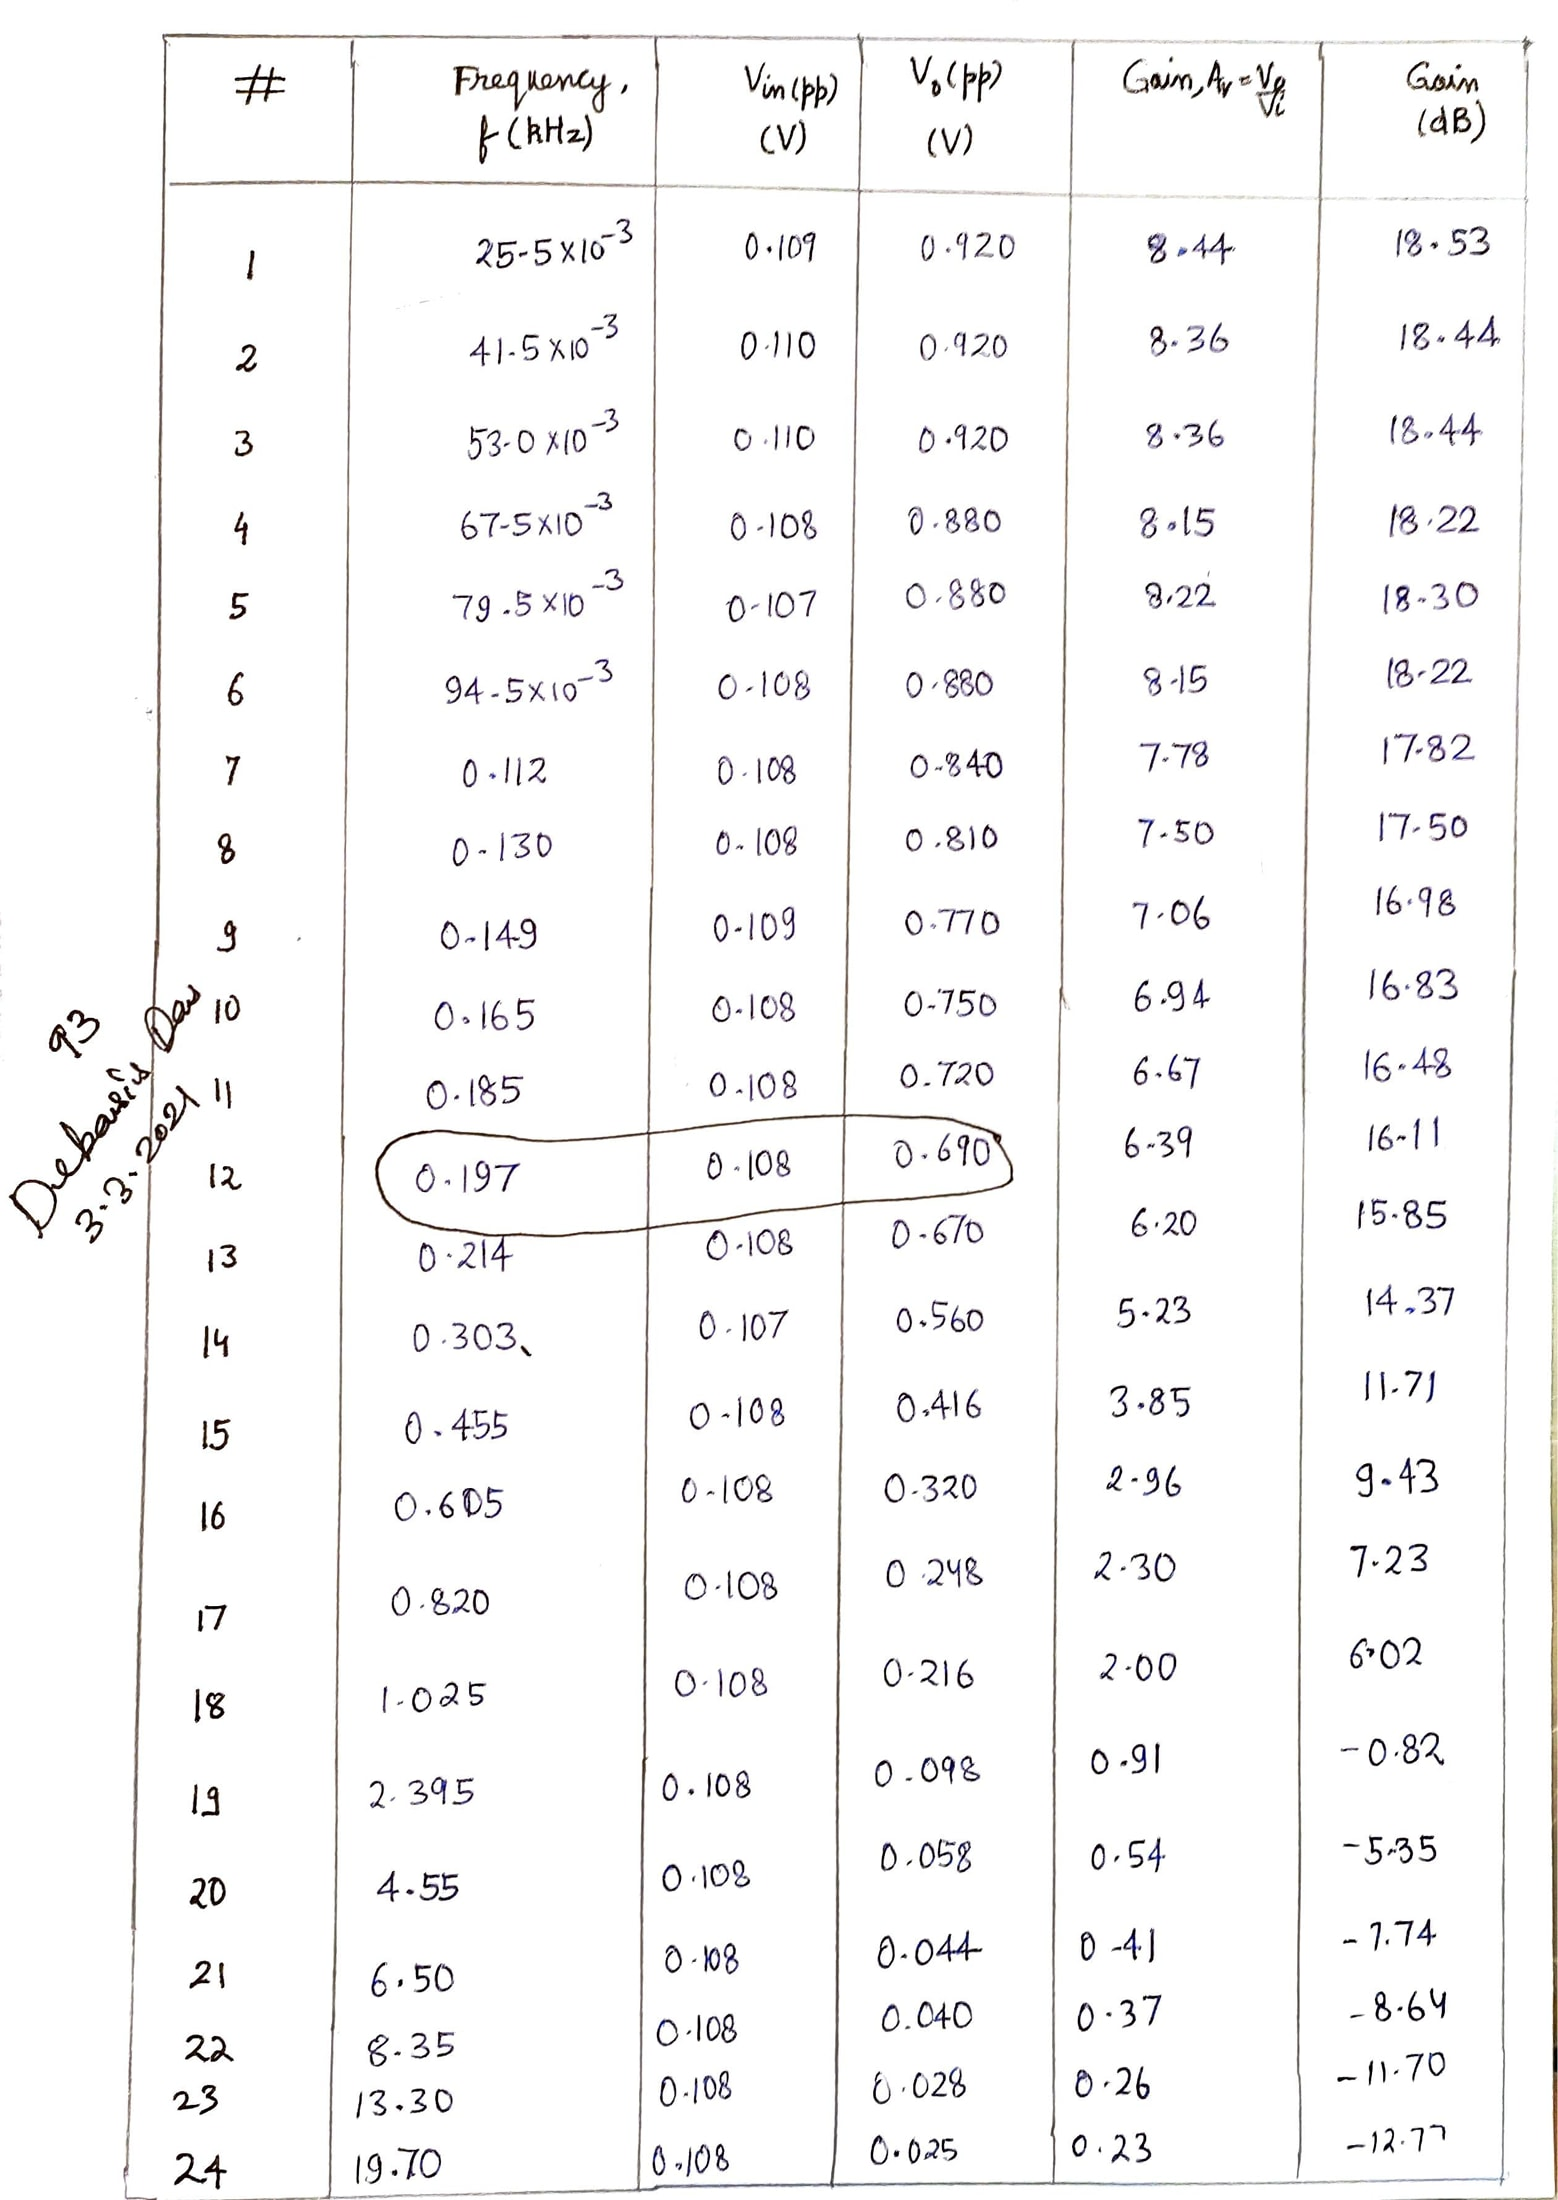
\includegraphics[scale = 0.25]{Documents/table.jpg}
\end{center}
\section{Graph}
\begin{center}
    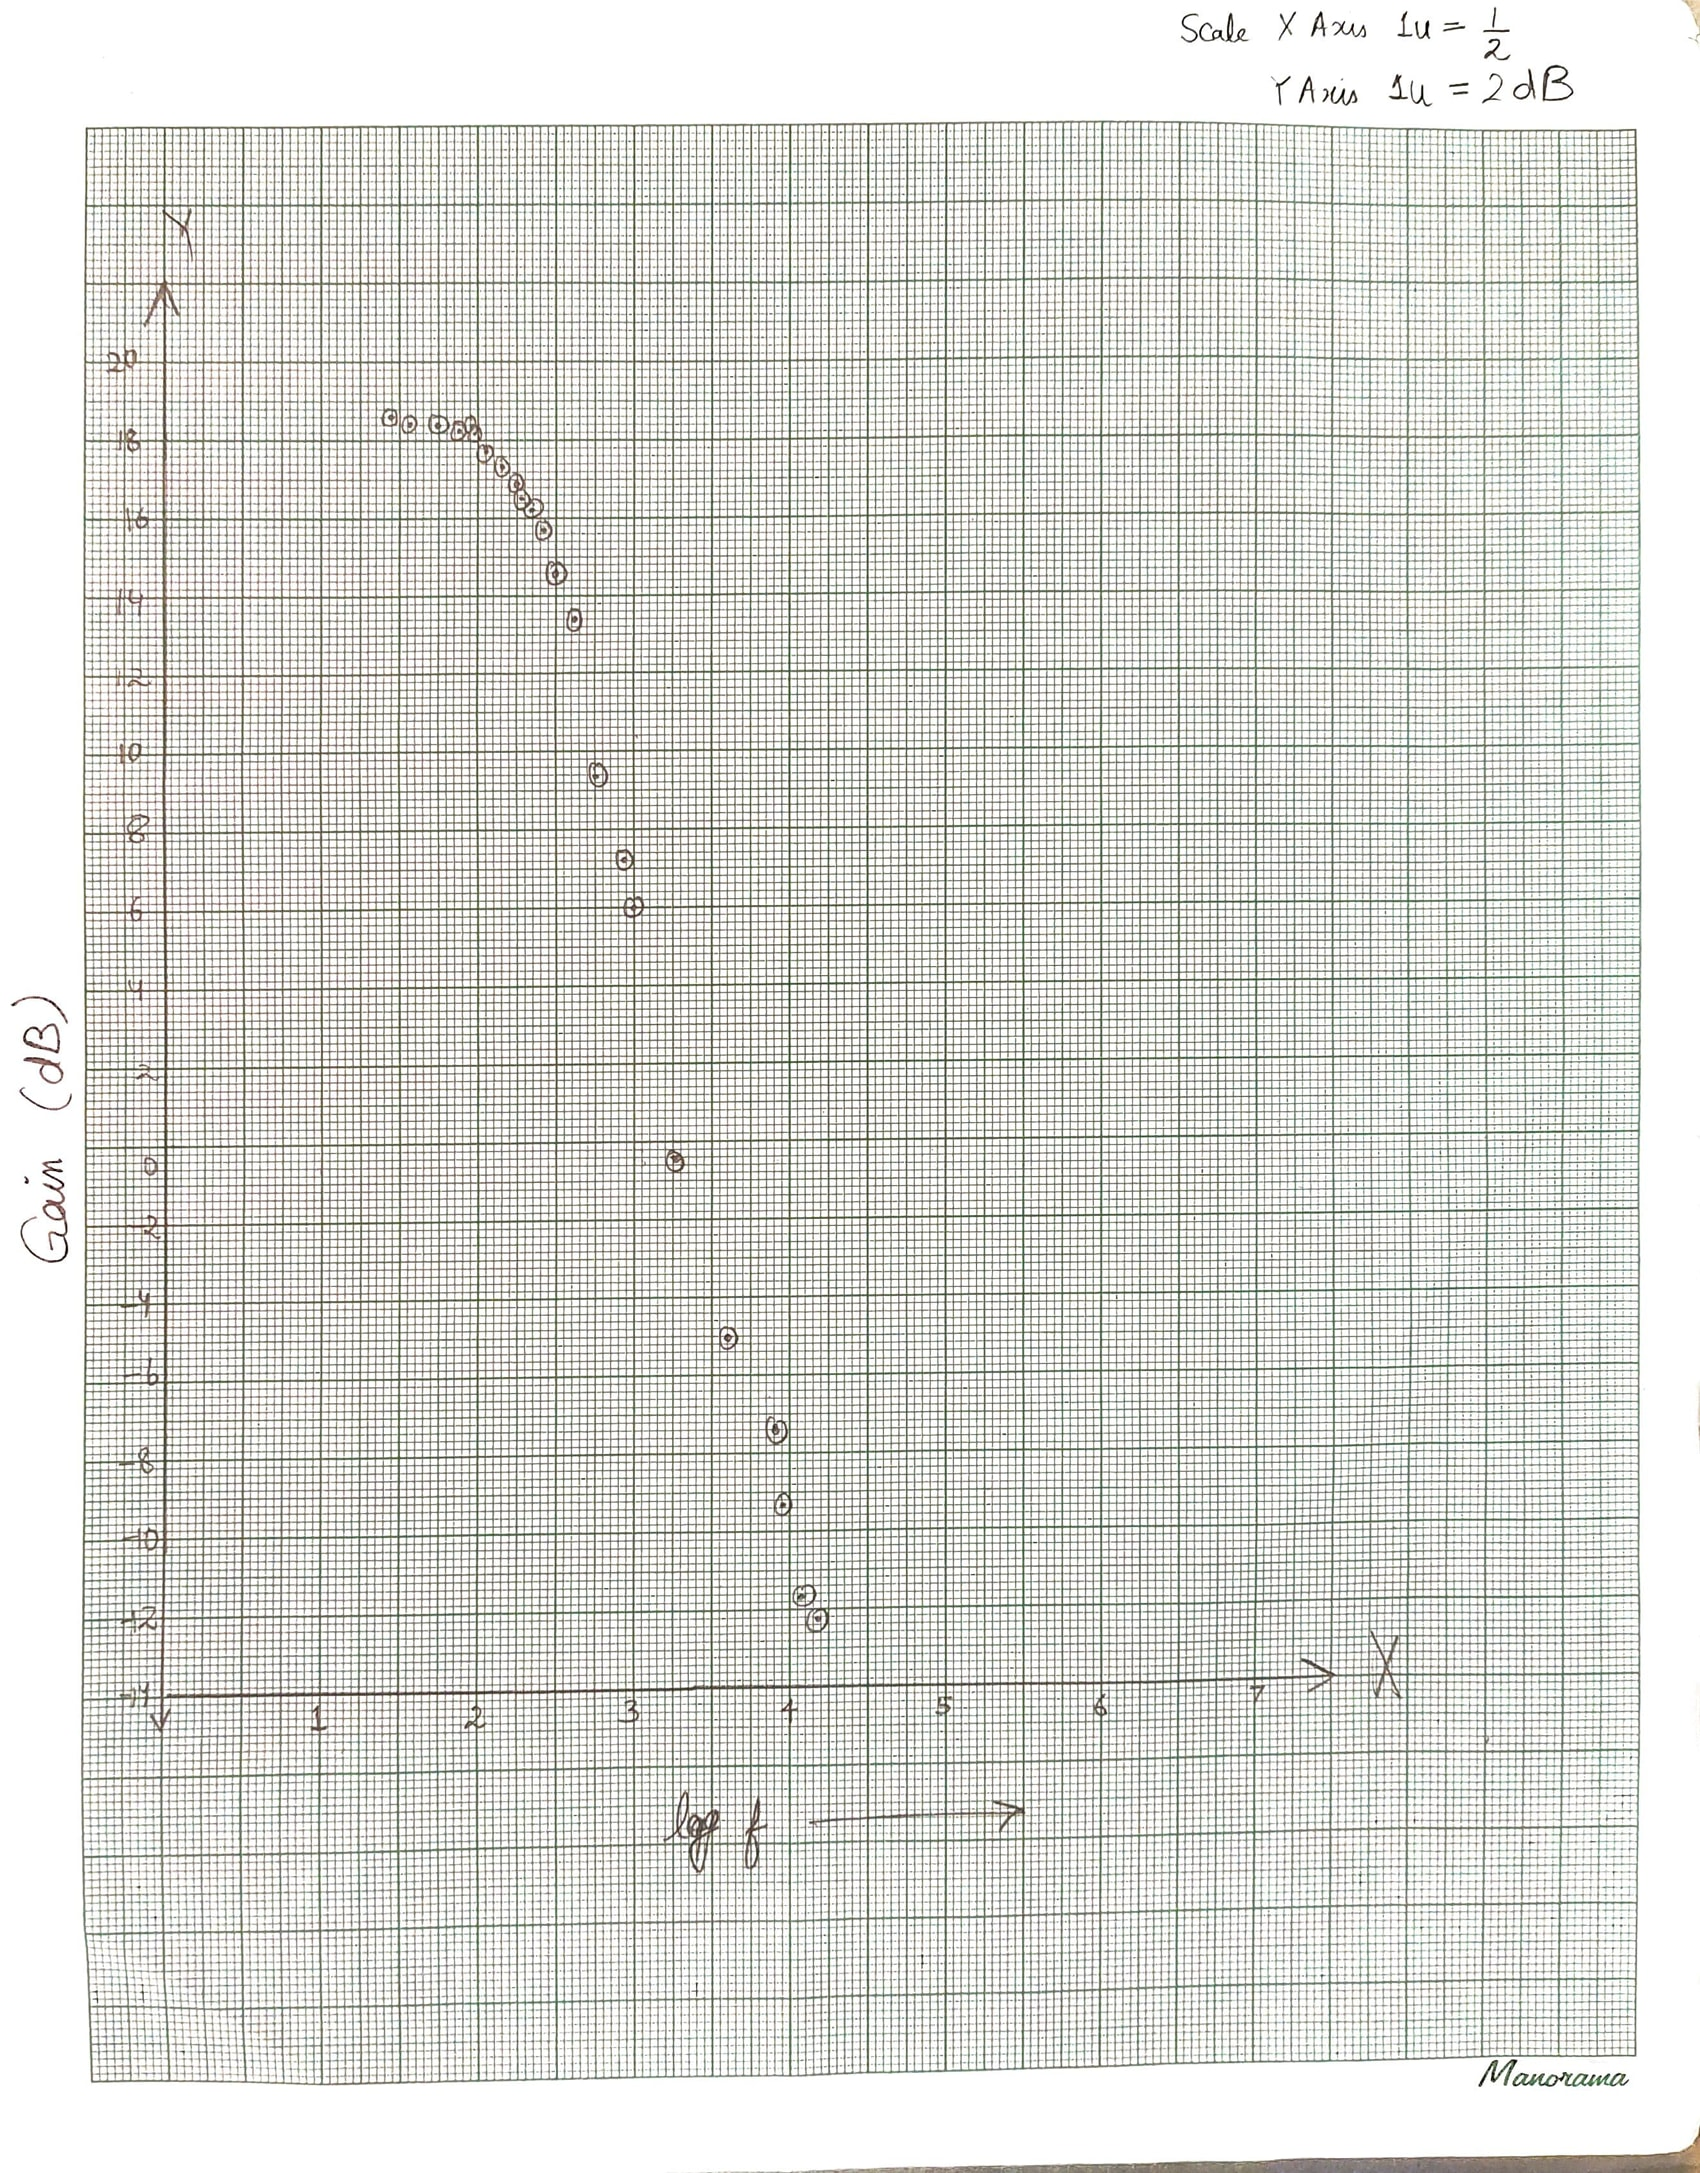
\includegraphics[scale = 0.27]{Documents/graph.jpg}
\end{center}
\section{Results}
\begin{enumerate}
    \item The integrator converts triangle wave into sine wave, sine wave into an inverted sine wave and square wave into a triangle wave.
    \item The differentiator converts triangle wave into a square wave, sine wave into an inverted sine wave and square wave into a delta-function type waveform.
    \item The active low pass filter constructed using the integrator circuit allows the waves of up to a certain frequency and beyond that frequency, the \emph{gain} falls down rapidly.
    \item The cut-off frequency obtained as a result of the experiment is $\SI{197}{\hertz}$.
\end{enumerate}
\section{Discussions}
\begin{enumerate}
    \item The integrator converts the triangle wave into a sine wave. This seems a bit a bit non-intuitive. Because triangle wave is a function made using linear functions so the integration of linear function must yield a parabolic curve. But the output waveform resembles a sinusoidal curve.
    \item The integrator converting square wave to triangle waves can be intuitively understood. A square wave has harmonics at all odd multiples of the fundamental, with strength diminishing as the number of the harmonic:
    \begin{center}
        $x_s(t) \simeq \sum_{n = 0}^\infty \frac{\cos 2 \pi (2n + 1) t}{2n + 1}$
    \end{center}
    \item A triangle wave is just the square wave, integrated:
    \begin{center}
        $x_\Delta(t) \simeq \sum_{n = 0}^\infty \frac{\sin 2 \pi (2n + 1) t}{(2n + 1)^2}$
    \end{center}
    \item A parabolic wave is the same thing, again:
    \begin{center}
        $x_p(t) \simeq \sum_{n = 0}^\infty -\frac{\cos 2 \pi (2n + 1) t}{(2n + 1)^3}$
    \end{center}
    \item Because of that cubic in the denominator, the difference between a sine wave and this "pseudo-sine" wave is very small. So the output waveform can be considered a sine wave.
    \item There is an apparent phase shift in all output wave forms which appears because of the input being in the inverting terminal.
    \item The differentiator circuit's output waveforms can easily understood by differentiating the input functions and obtaining the output functions.
    \item The \emph{gain} in the active low pass filter scenario even dips into negative values. The term \emph{negative gain} is reserved for those cases where the line has a downward slope and so reverses the polarity of the signal (a $180 \degree$ phase change). An Op-Amp in an inverting configuration is a prime example which we have used in the set-up.
    \item Similarly, we can construct an active high pass filter with the help of a differentiator circuit and using a low pass filter and high pass filter, a band pass filter can be constructed which will allow a range of frequency to pass, which can be set to our convenience. 
\end{enumerate}
\section{Error Analysis}
\begin{enumerate}
    \item The integrator and differentiator circuits were qualitative experiments so no error analysis can be realised.
    \item The calculated cut-off frequency for the active low pass filter is $\SI{197.47}{\hertz}$. The frequency as obtained from the graph is $\SI{197}{\hertz}$. Therefore, 
    \begin{center}
         Percentage error = $\dfrac{197.47-197}{197.47}\times 100 \% = 0.24\%$
    \end{center}
\end{enumerate}
\section{Conclusion}
\begin{enumerate}
    \item All results obtained are in accordance to the expectations.
    \item The errors are quite small and are due to elements of the circuit.
    \item The active low pass filter works as expected.
    \item The differentiator and integrator circuits can be used in analog computers, analog-to-digital converters and wave-shaping circuits.
\end{enumerate}